\chapter{Comparisons of model performances on various datasets} 
\label{chap_comparisons} 

This chapter synthesizes results of reconstructions by the proposed models to compare their performances. Comparisons are shown for streamwise velocities from both DNS datasets of isotropic turbulence (section \ref{sec:data_isotropic}) and channel flow (section \ref{sec:data_channel}). Isotropic turbulence is rather ideal yet retains the fundamental characteristics of real turbulent flows. It facilitates all computations of proposed methods for its homogeneity and periodicity. The data of turbulent channel flow mimics better real flows. Results on these data can be generalized for other velocity components and for experimental data. 

We study the setup where multi-source measurements are given, the HTLS and LTHS, as described in section \ref{sec:probdef2}. For each data, three favorable configurations of balanced energy losses in space and time are used to perform detailed analyses. These configurations permit to apply both families of approaches, the empirical models to learn the relation between large and small scales, and the fusion models to combine the two sources. With empirical approaches such as regressions (chapter \ref{chap_linearregression}) or dictionary learning (chapter \ref{chap_dictionarylearning}), LTHS planes are considered as training samples, while HTLS measurements are used for reconstruction. Fusion models instead simultaneously combine both sources of measurements by either exploiting different hypotheses (chapter \ref{chap_NLM} and \ref{chap_BayesianFusion}). 

Comparisons between two families of methods are valid but bias. Empirical mapping models are not designed to take benefits of information in time, and reconstruction errors purely depend on the subsampling ratio in space. Performances of fusion models will depend on both ratios in space and time. Both results from the two proposed models suggest that more gains are expected when the subsamplings are in a balanced manner. In such cases, the models can get benefits from both sources of information. Otherwise, if the loss caused by one subsampling is much more severe than by another, the models tend to perform at best as accurate as the single interpolation from measurements with the lower energy loss. Comparisons with regression models and dictionary learning also demonstrate how information from the measurements in time are beneficial in improving reconstruction accuracies.

Dictionary learning is omitted in all the analyses, since it works only when downsampled fields are considered. This configuration is different from all other chapters and the inspired experiment at LML. For the direct subsampling cases, it shows no improvement compared to spatial interpolations.


\section{Reconstruction results on DNS data of isotropic turbulence}
\label{sec:comparisons_isotropic}
Detailed analyses of proposed models are investigated on the DNS data of isotropic turbulence as described in section \ref{sec:data_isotropic}. The data facilitates numerical experiments of all proposed methods for its isotropy, periodicity and homogeneity. The computation complexity is first discussed. Then, detailed analyses of model performances are shown for the three cases of balanced energy losses. 

\subsection*{Computation time}
All numerical experiments of the proposed methods are performed on the same personal computer using either Matlab (verion \textit{2014b}) or python (version $ 2.7 $). NLM propagation models are programmed in $ C $ using \textit{openMP} parallelization. Dictionary learning codes are based on \textit{SPArse Modeling Software} (SPAM) package (\url{http://spams-devel.gforge.inria.fr/}). This package is written in $ C $ with Matlab and python interfaces. Regression codes are based on \textit{scikit-learn} package \citep{scikit-learn}. The data contains $ 37 \times 96 $ HR planes at the resolution $ 96 \times 96 $ (about $ 400 $ Mb, extracted from $ 25 $ Gb of original simulation data).

Regression and Bayesian fusion models are the simplest and fastest model to test. To reconstruct all $ 37 \times 96 $ fields, Bayesian fusion model takes only a few minutes to interpolate, learn the covariance matrices and perform the weighted sum, thanks to the matrix vectorization. Regression models, both RR and KRR, take up to one minute to train the models. The time to reconstruct the whole $ 37 \times 96  $ fields is about $ 1 \sim 2 $ minutes. The most time consuming step is the cross-validation, which takes about $ 10 \sim 30 $ minutes. Coupled dictionary learning takes up to about $ 10 $ seconds to reconstruct one field in the case of \textit{SR3} (see table \ref{tab:DLapproaches}) and even faster with \textit{SR1} and \textit{SR2}. The learning step, which is more expensive, can be done \textit{offline}. Learning a dictionary of size $ K = 2 \times 16^2 $ from $ m=10^5 $ patches of the dimension $ \dimpsh = 16^2 $ takes about one hour to converge. With NLM-based propagation models, the estimation of one field takes about $ 1 \sim 2 $ seconds without parallelization. All methods acquire a tractable computational time and therefore could be generalized to larger experiments. To recall, all codes and data are available at \url{https://github.com/linhvannguyen/PhDworks/}.

\subsection*{Model performance analyses}
\begin{table} 
	\caption{\label{tab:comparisons_various_cases}
	Isotropic turbulence: configuration parameters of three testing cases with balanced energy losses. The subsampling ratios of HTLS measurements are $ \sqrt{\dimsh /\dimsl } $ and equal in both spatial directions. The ratios of LTHS measurements in time (streamwise in this case) are $ \dimth/\dimtl $. The normalized energy losses in space $\Delta\kappa_s$ and in time $\Delta\kappa_t$ are defined in Eq.~(\ref{eq:RMS_losses}).}
	\vspace{.5cm}
	\centering
	\begin{tabular}{ccS[table-format=1.0]S[table-format=1.0]cS[table-format=1.2]S[table-format=1.2]} 
		\toprule
		\multirow{2}{*}{Case}&\multicolumn{1}{c}{}&\multicolumn{2}{c}{Subsampling ratios}&\multicolumn{1}{c}{}&\multicolumn{2}{c}{Energy losses}\\ 
		\cmidrule{3-4} \cmidrule{6-7}
		 & & {$\sqrt{\dimsh /\dimsl }$} & $\dimth/\dimtl$ & & {$\Delta\kappa_s(\%)$} & {$\Delta\kappa_t (\%)$}\\ 
		\midrule 
		5 &  & 3  & 4 & & 1.03 & 1.23 \\ %\addlinespace	 
		6 &  & 4  & 6 & & 2.63 & 3.56 \\ %\addlinespace
		7 &  & 6  & 8 & & 7.29 & 6.53 \\ %\addlinespace
		\bottomrule
	\end{tabular}
\end{table}

We study three cases of balanced energy losses in space (spanwise and vertical direction) and time, with of subsampling ratios and energy losses are summarized in table \ref{tab:comparisons_various_cases}. Due to the lack of time-resolved fields, the streamwise direction is also considered as the virtual time direction. The first family of methods (regression and dictionary learning) does not depend on this condition. Bayesian fusion model also depends on the losses of energy but not really the properties of the flow in time. NLM model might be more sensitive, since the rapid distortion assumption is stronger with convective flows. It is expected to work better in the case where time-resolved sequence of snapshots are studied.

\begin{table}
\caption{\label{tab:comparisons_results}
NRMSEs of all scales reconstruction errors for three cases in table \ref{tab:comparisons_various_cases}. $\overline{\epsilon}$ and $\epsilon_{max}$ are the mean and max NRMSE defined in Eq.~(\ref{eq:NRMSE}). $\overline{\epsilon}$ is averaged over all fields, while $\epsilon_{max}$ is computed for the most difficult positions in space and time (the most remote from all nearby measurements). The smallest errors in each cases are boldfaced.}
\vspace{.5cm}
\centering
	\begin{tabular}{lcccccccc} 
		\toprule \multirow{2}{*}{Method}&\multicolumn{1}{c}{}&\multicolumn{3}{c}{$\overline{\epsilon}$}&\multicolumn{1}{c}{}&\multicolumn{3}{c}{$\epsilon_{max}$}\\
		\cmidrule{3-5} \cmidrule{7-9}
		 & & {Case 5} & {Case 6} & {Case 7} & & {Case 5} & {Case 6} & {Case 7}\\
		\midrule 
		$ \Interp_s \y $ & & 0.19 & 0.28 & 0.43 & & 0.22 & 0.35 &  0.52 \\ 
		$ \Interp_t \x $ & & 0.13 & 0.23 & 0.31 & & 0.19 & 0.28 &  0.42 \\ 	\midrule 
		RR & & 0.14 & 0.23 & 0.35 & & 0.20 & 0.34 &  0.50 \\
		KRR & & 0.13 & 0.23 & 0.34 & & 0.20 & 0.34 &  0.49 \\ 	\midrule 
		Greedy propagation & & 0.11 & 0.20 & 0.32 & & 0.18 & 0.33 &  0.51 \\
		Non-greedy propagation & & 0.11 & 0.19 & 0.30 & & 0.17 & 0.31 &  0.46 \\	
		Fusion (LG)  & & 0.11 & 0.18 & 0.27 & & 0.17 &  0.26 &  0.41 \\
    	Fusion (BF)  & & 0.11 & 0.18 & 0.26 & & 0.17 &  0.26 &  0.40 \\ \midrule 
    	\myrowcolour
    	Best scores  & & \textbf{0.11} & \textbf{0.18} & \textbf{0.26} & & \textbf{0.17} &  \textbf{0.26} &  \textbf{0.40} \\ \bottomrule
	\end{tabular}
\end{table}

Table \ref{tab:comparisons_results} gathers NRMSEs between reconstructed and reference fields of three cases in table \ref{tab:comparisons_various_cases}. Both average and maximum errors are shown for all methods. Interpolations are 2D in space as $ \Interp_s \y $ and 1D in time as $ \Interp_t \x $. Regression models are either linear (RR) or non-linear (KRR) using RBF kernel. NLM-based propagations of both greedy and non-greedy schemes are shown. As fusion models, linear Gaussian or Bayesian fusion of non-informative prior are studied. The ``best scores'', i.e. lowest NRMSEs, are shown in bold at the bottom row. Fusion models by combining all sources of measurements give lowest errors. The accuracy improvements compared to single interpolations are significant. $ \bar{\epsilon} $ is reduced by $ 15 \% \sim 25\% $, and $ \epsilon_{max} $ is reduced $ 5\% \sim 10\%$ compared to the best single interpolation. 

Performances of fusion and NLM-based propagation models are similar at the low subsampling ratio (case 5). Fusion models are superior in cases 6 and 7 of higher ratios. They take into account all sources of measurements and find the best compromise estimates via weighted sums. NLM models propagate small-scale information from LTHS planes and put on top of initial spatial interpolations. The quality of propagations strongly depends on flow dynamics. When the distance between the LTHS planes is far, the assumption that small scales are advected by large ones can be rather crude.

Regression models give worse results than almost all methods except spatial interpolations. As discussed, their errors depends solely on the subsampling ratio in space. All regression models are not designed in such way to take benefits from information in time. LTHS planes are used only to train the models. The models use averaged coefficients to reconstruct all fields regardless the temporal dynamics of the flows. The performances should be compared only to the spatial interpolation $ \Interp_s \y $. KRR gives slightly better reconstructions to RR. The model reduces $ \bar{\epsilon} $ by $ 18\% \sim 32\% $, and $ \epsilon_{max} $ by $ 5\% \sim 10\% $ compared to interpolations. 

Cases 5 and 7 are used to further analyze model performances. Case 5 corresponds to small energy losses due to subsamplings in both time (streamwise) and space (about $ 1 \% $), while these losses of case 7 are more severe (about 7 $ \% $). The configuration with small losses is favorable for all models, and should be of interest when designing experiments such that the reconstructed information is reliable. Case 7 is more critical to highlight different behaviors and also limitations of present approaches.

\begin{figure}
\begin{center}
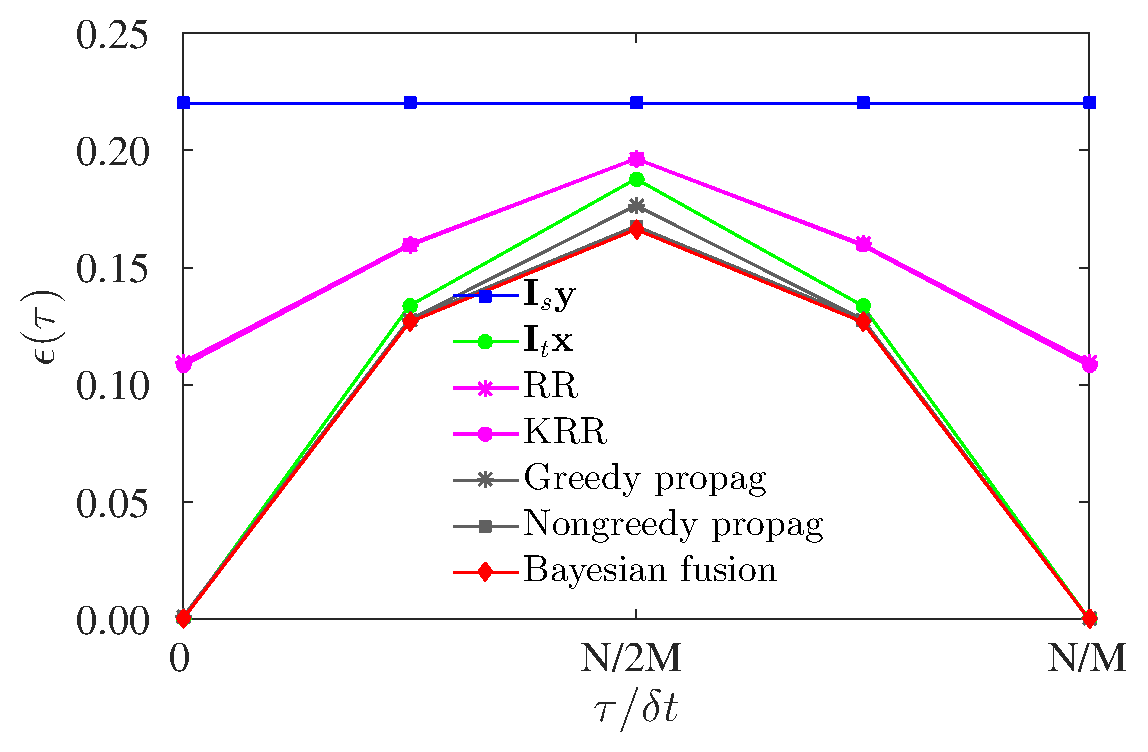
\includegraphics[width = 0.7\columnwidth]{./images/comparisons/isotropic/compare_NRMSE_time_middlepoints_sspacing3_tspacing4.eps}
\caption{\label{fig:final_isotropic_error_time_case5} Isotropic turbulence: NRMSEs are functions of time distances from the previous LTHS instant at the most difficult spatial location, i.e. at $ (\Delta y/2,\Delta z/2,\tau) $. These errors are estimated between reference and reconstructed streamwise velocities by spatial and temporal interpolations, RR, KRR, non-greedy propagation and Bayesian fusion models. Results are shown for case 5 in table \ref{tab:comparisons_various_cases}, with the subsampling ratios $ \dimth/\dimtl = 4 $ in time and $ \dimsh/\dimsl = 3 \times 3 $ in space.}
\end{center}
\end{figure}

\begin{figure}
\begin{center}
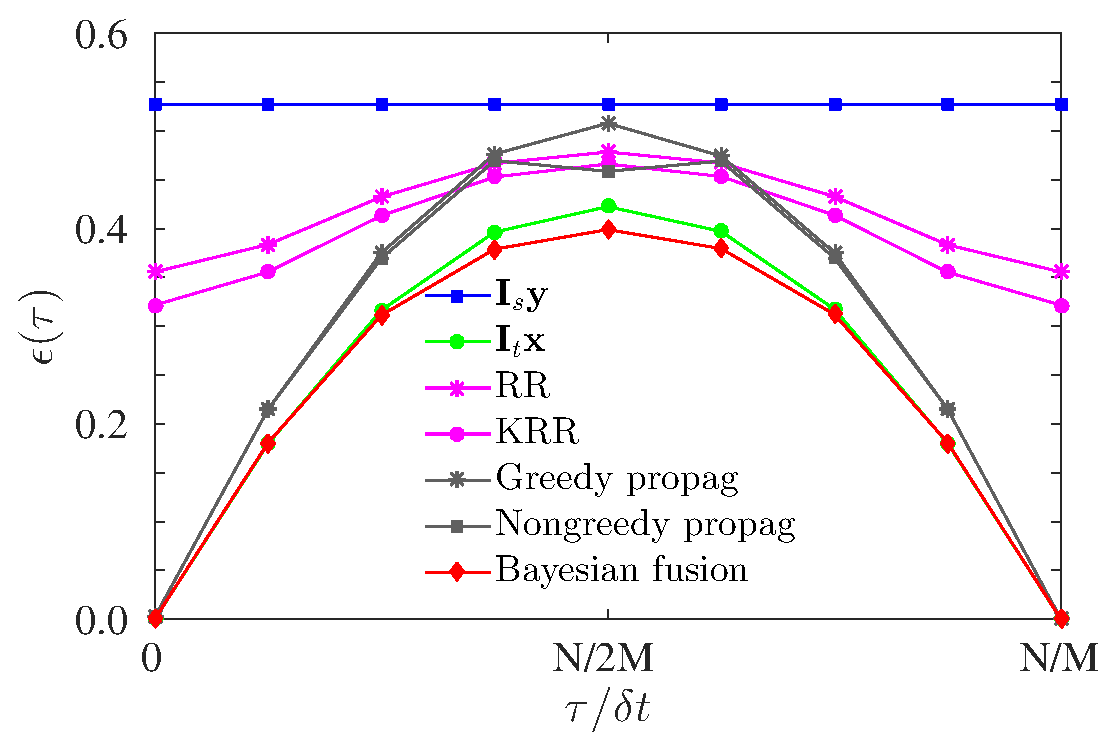
\includegraphics[width = 0.7\columnwidth]{./images/comparisons/isotropic/compare_NRMSE_time_middlepoints_sspacing6_tspacing8.eps}
\caption{\label{fig:final_isotropic_error_time_case7} Isotropic turbulence: similar plot as figure \ref{fig:final_isotropic_error_time_case5} for case 7 in table \ref{tab:comparisons_various_cases}, with the subsampling ratios $ \dimth/\dimtl = 8 $ in time and $ \dimsh/\dimsl = 6 \times 6 $ in space.}
\end{center}
\end{figure}

\begin{figure}[h]
\begin{center}
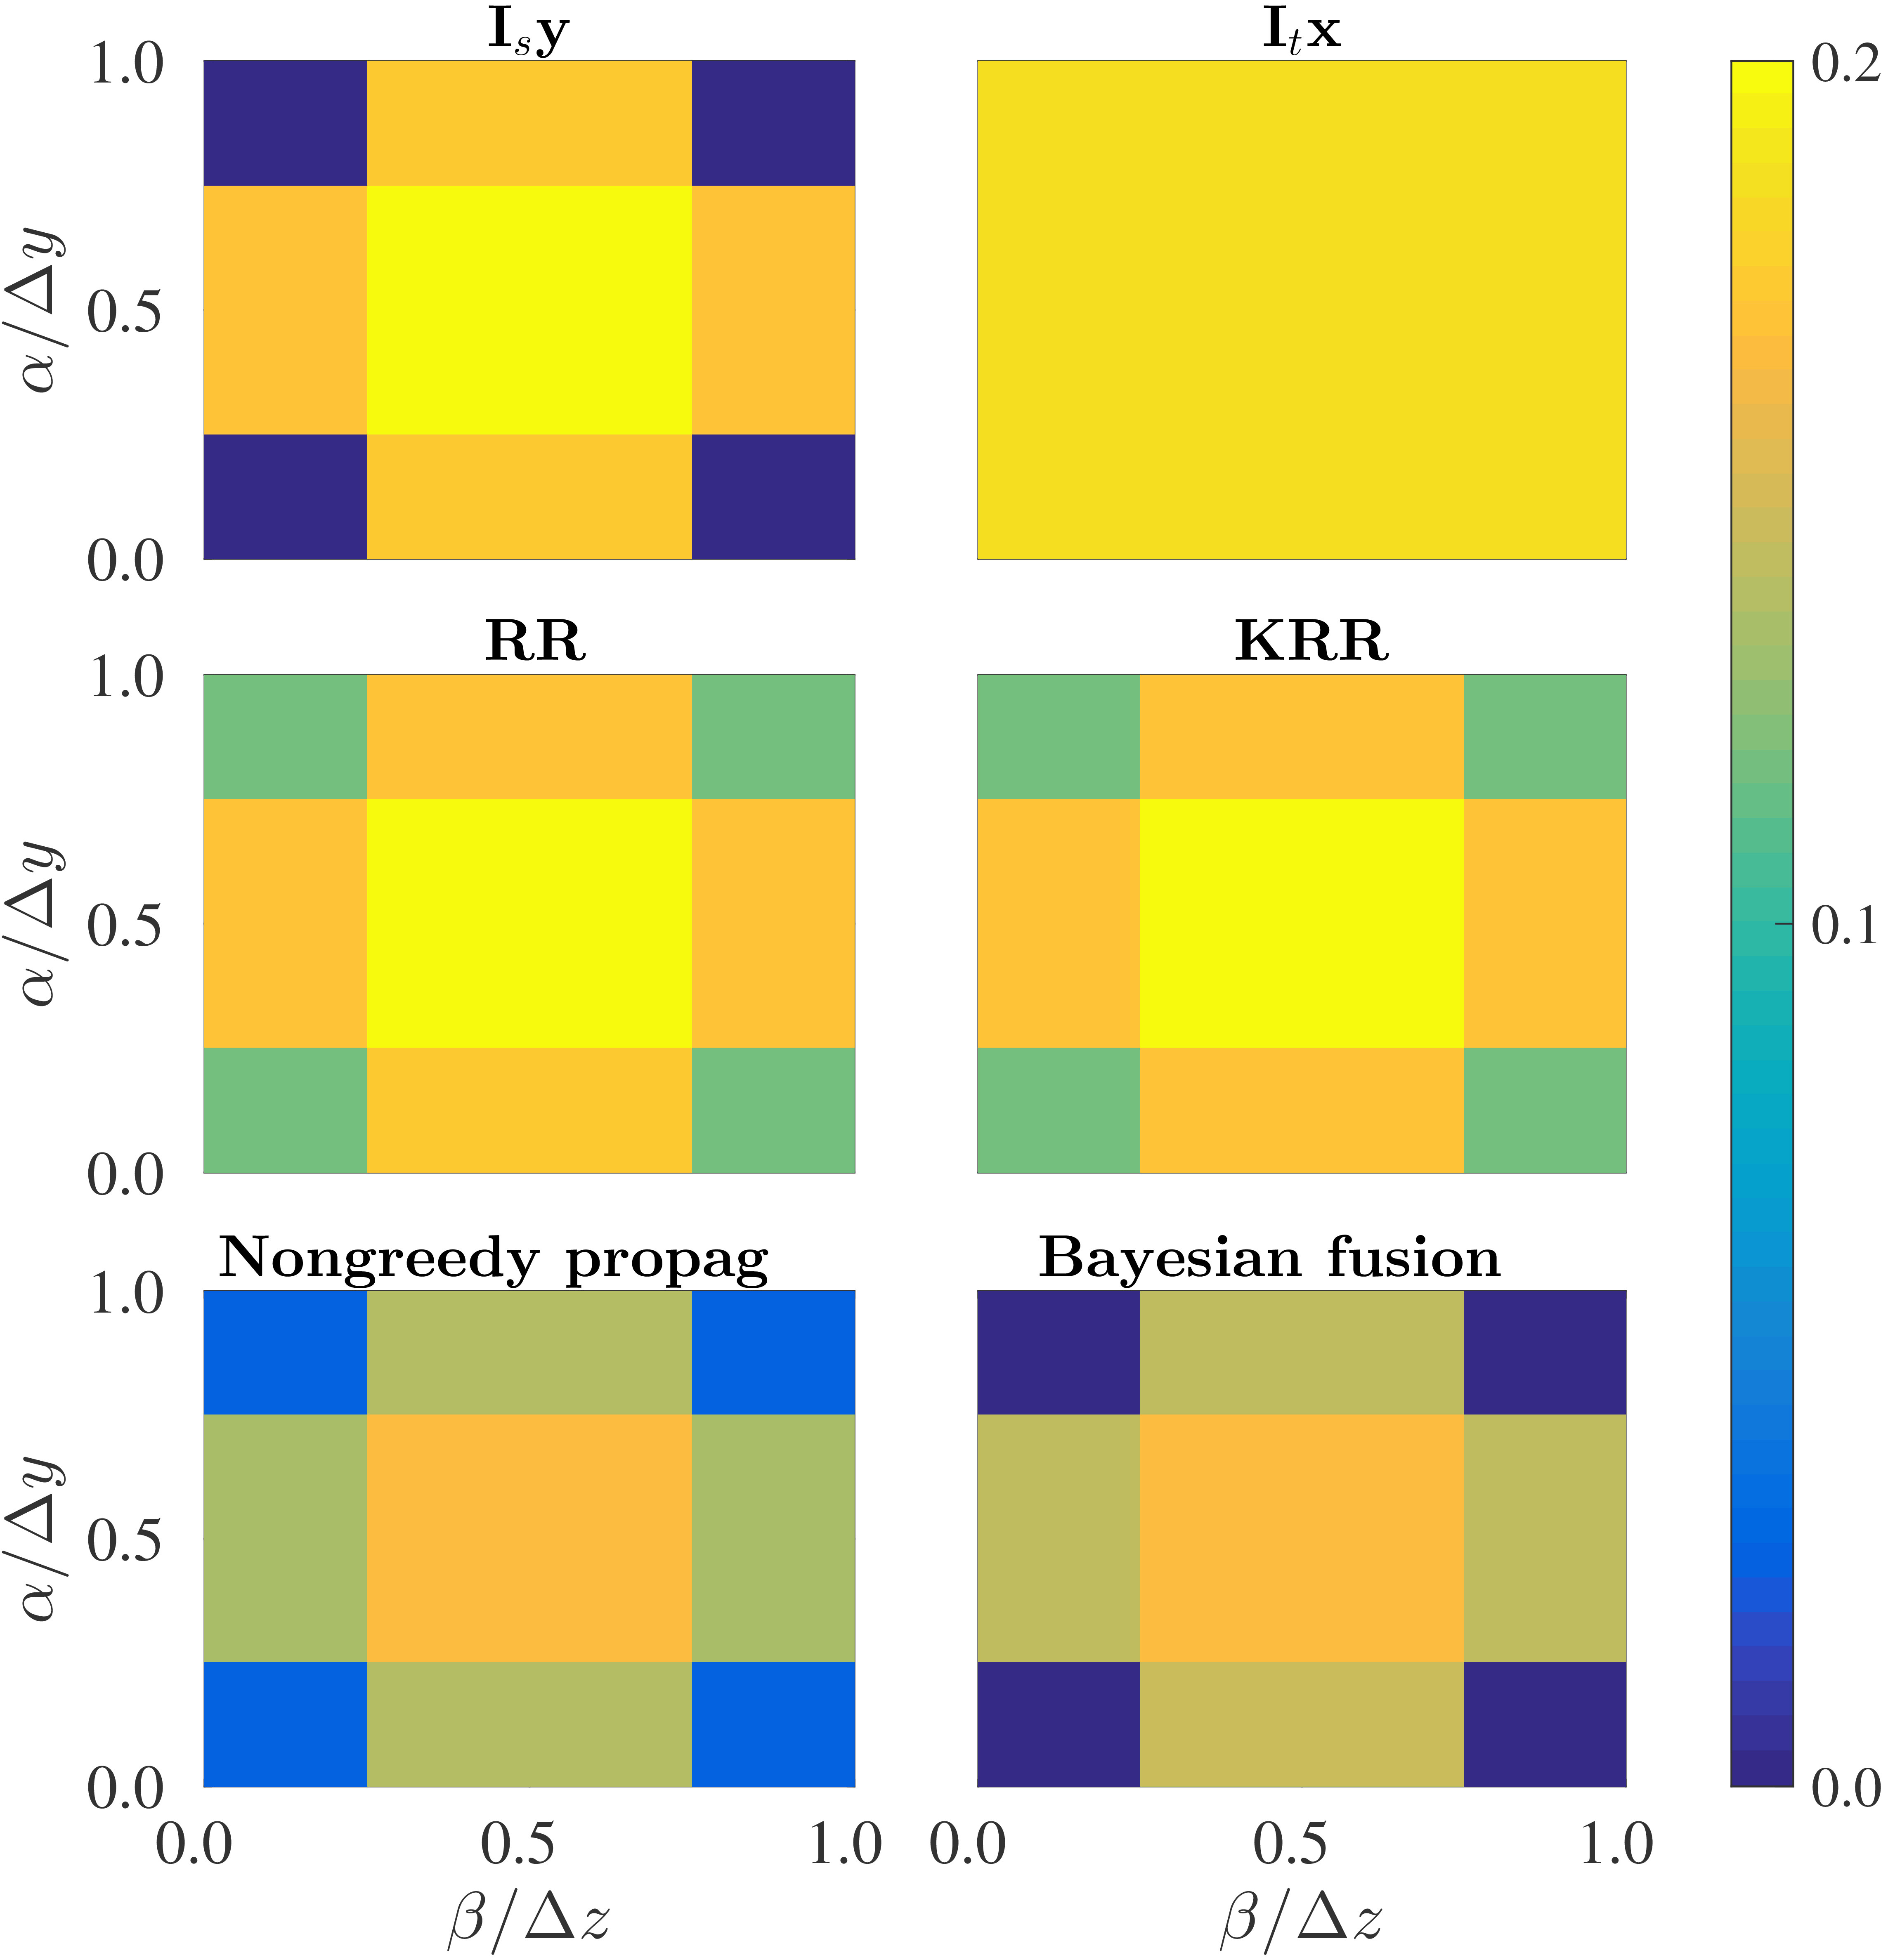
\includegraphics[width = 0.8\columnwidth]{./images/comparisons/isotropic/compare_boxin4HWs_sspacing3_tspacing4.png}
\caption{\label{fig:final_isotropic_error_boxes_case5} Isotropic turbulence: NRMSEs are functions of spatial coordinates in an element block at the most difficult instant, i.e. at $ (\alpha,\beta,\dimth \delta t/2\dimtl) $. These errors are estimated between reference and reconstructed streamwise velocities by spatial and temporal interpolations, RR, KRR, non-greedy propagation and Bayesian fusion models. Results are shown for case 5 in table \ref{tab:comparisons_various_cases}, with subsampling ratios of $ \dimth/\dimtl = 4 $ in time and $ \dimsh/\dimsl = 3 \times 3 $ in space.}
\end{center}
\end{figure}

\begin{figure}[h]
\begin{center}
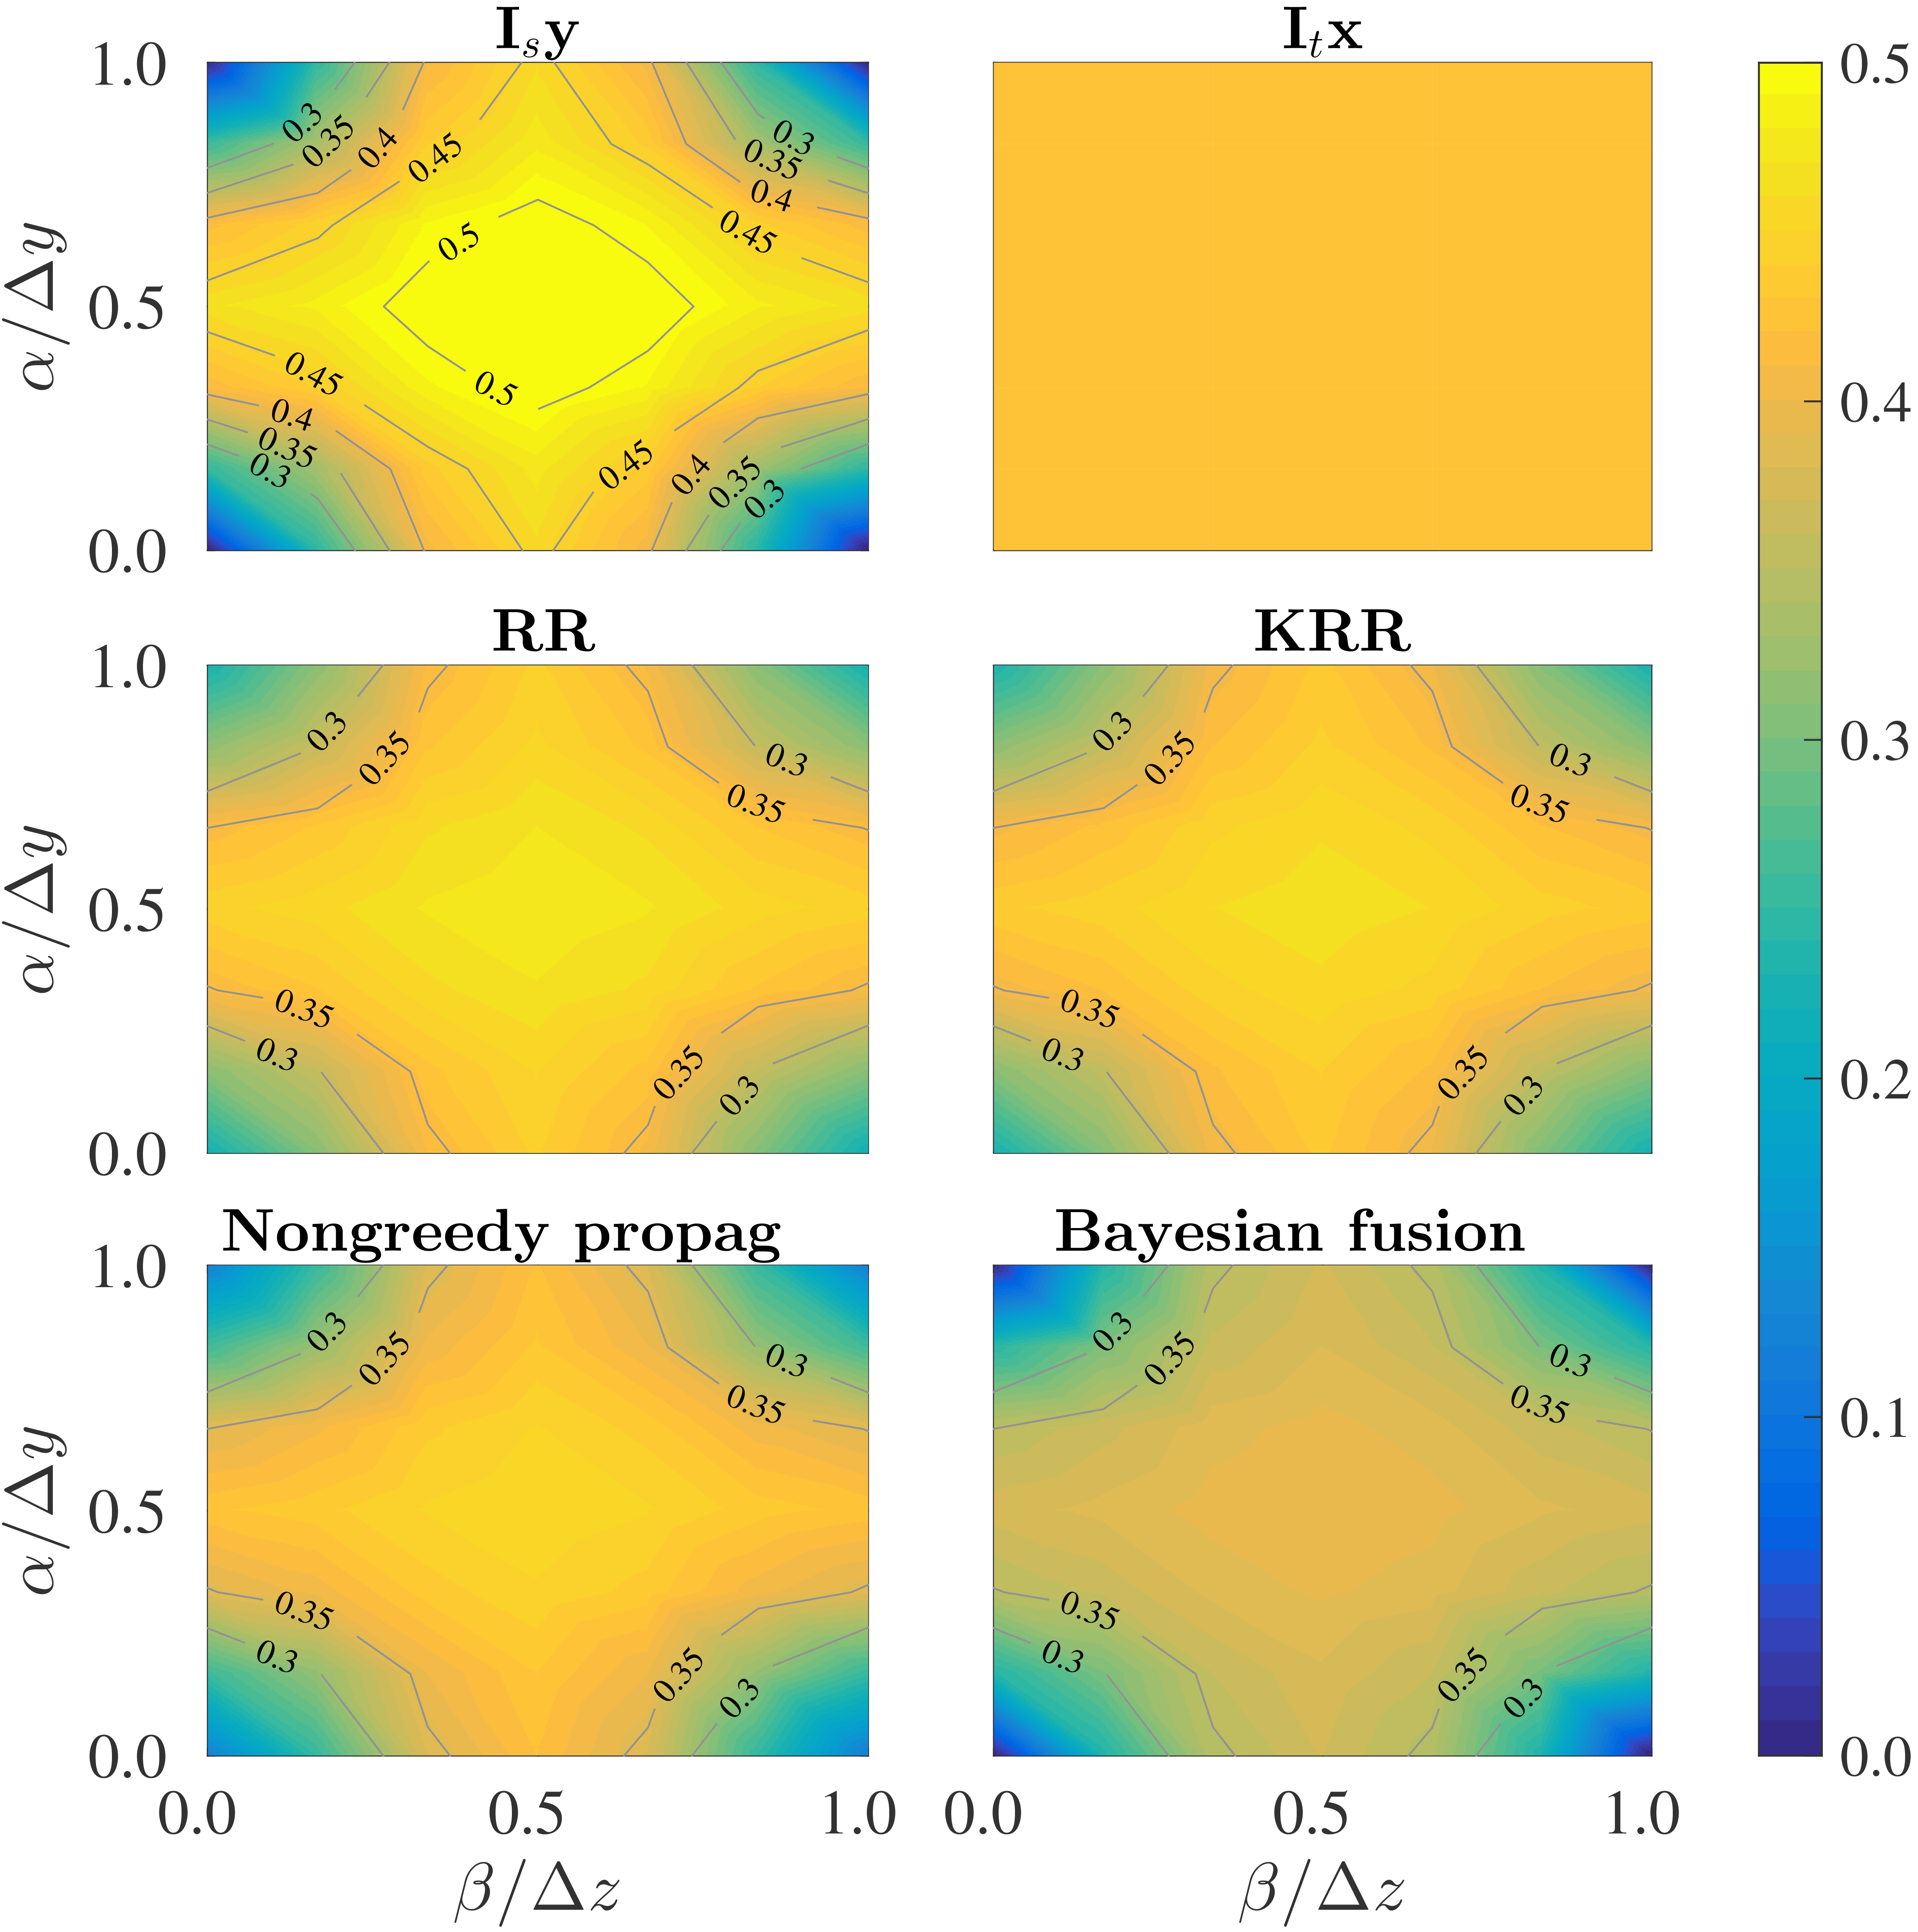
\includegraphics[width = 0.8\columnwidth]{./images/comparisons/isotropic/compare_boxin4HWs_sspacing6_tspacing8.png}
\caption{\label{fig:final_isotropic_error_boxes_case7} Isotropic turbulence: NRMSEs are functions of spatial coordinates as in figure \ref{fig:final_isotropic_error_boxes_case5}. Results are shown for case 7 in table \ref{tab:comparisons_various_cases}, with subsampling ratios of $ \dimth/\dimtl = 8 $ in time and $ \dimsh/\dimsl = 6 \times 6 $ in space.}
\end{center}
\end{figure}

To analyze the reconstructions in time, figure \ref{fig:final_isotropic_error_time_case5} shows NRMSEs as a function of distances $ \tau $ from the previous LTHS time step in cases 5. For each $ \tau $, NRMSE is estimated using the set of point $ \varmathbb{J}$ including points at local coordinates $ (\Delta y/2,\Delta z/2, \tau) $ of all blocks used to estimate $ \epsilon_{max} $. NRMSEs are small close to the LTHS measurements ($ \tau/\delta t=0 $ and $ \tau/\delta t=\dimth/\dimtl $) and increase when moving toward the middle ($ \tau/\delta t=\dimth/2\dimtl $). Spatial interpolation behaves differently since the NRMSE is independent of time. Regression models illustrate the advantages of learning a model by significantly reducing the errors (about $ 15 \% $ for mid-planes at $ \dimth/\dimtl $) compared to spatial interpolation. Time interpolation gives smaller error than RR and KRR, since those errors of regression models depend only on the subsampling ratio in space. These temporal information from LTHS planes are taken into account to further improve the reconstruction using fusion models. Both the propagation models and fusion model give better reconstructions than all other models. Bayesian fusion and non-greedy model are slightly better than the greedy one.

Figure \ref{fig:final_isotropic_error_time_case7} shows similar results as in figure \ref{fig:final_isotropic_error_time_case5} for case 7 with very severe subsampling ratios in both space and time. Model performances are consistent with case 5, except that propagation models now give higher NRMSEs than time interpolation. This is because the propagation models start from a critical loss of information and could not recover completely. Also, this approach does not take advantages of temporal information from LTHS snapshots (except their small scales to propagate). Bayesian fusion model, which proposes a compromise estimate between the two interpolations. The model yields the minimum errors at all time steps. Even in the middle of two LTHS instants, the maximum fusion error remains lower than the one obtained with both interpolations. 

To analyze the reconstructions in space, figures \ref{fig:final_isotropic_error_boxes_case5} and \ref{fig:final_isotropic_error_boxes_case7} show spatial NRMSE maps by all the methods as a function of local coordinates $ (\alpha,\beta) $ as described in figure \ref{fig:element_block}, section \ref{sec:probdef2}. For each $ (\alpha,\beta) $, NRMSE is estimated using equation~(\ref{eq:NRMSE}), where $ \varmathbb{J} $ includes points at $ (\alpha,\beta,\dimth \delta t/2 \dimtl) $ of all blocks used to estimate $ \epsilon_{max} $. All methods give small NRMSEs close to the four HTLS positions in the corners. The errors increase when approaching the center. Time interpolation behaves differently since the errors are independent of spatial coordinates. Compared to interpolation in space, regression models do not give exact estimates at the HTLS positions. However, errors far from these four points are significantly reduced. The fusion models yields the best reconstruction results, where the Bayesian fusion model yields the smallest errors at all positions. At the most difficult positions (near the center of the block), it improves the reconstruction significantly compared to other methods. 


\begin{figure}
\begin{center}
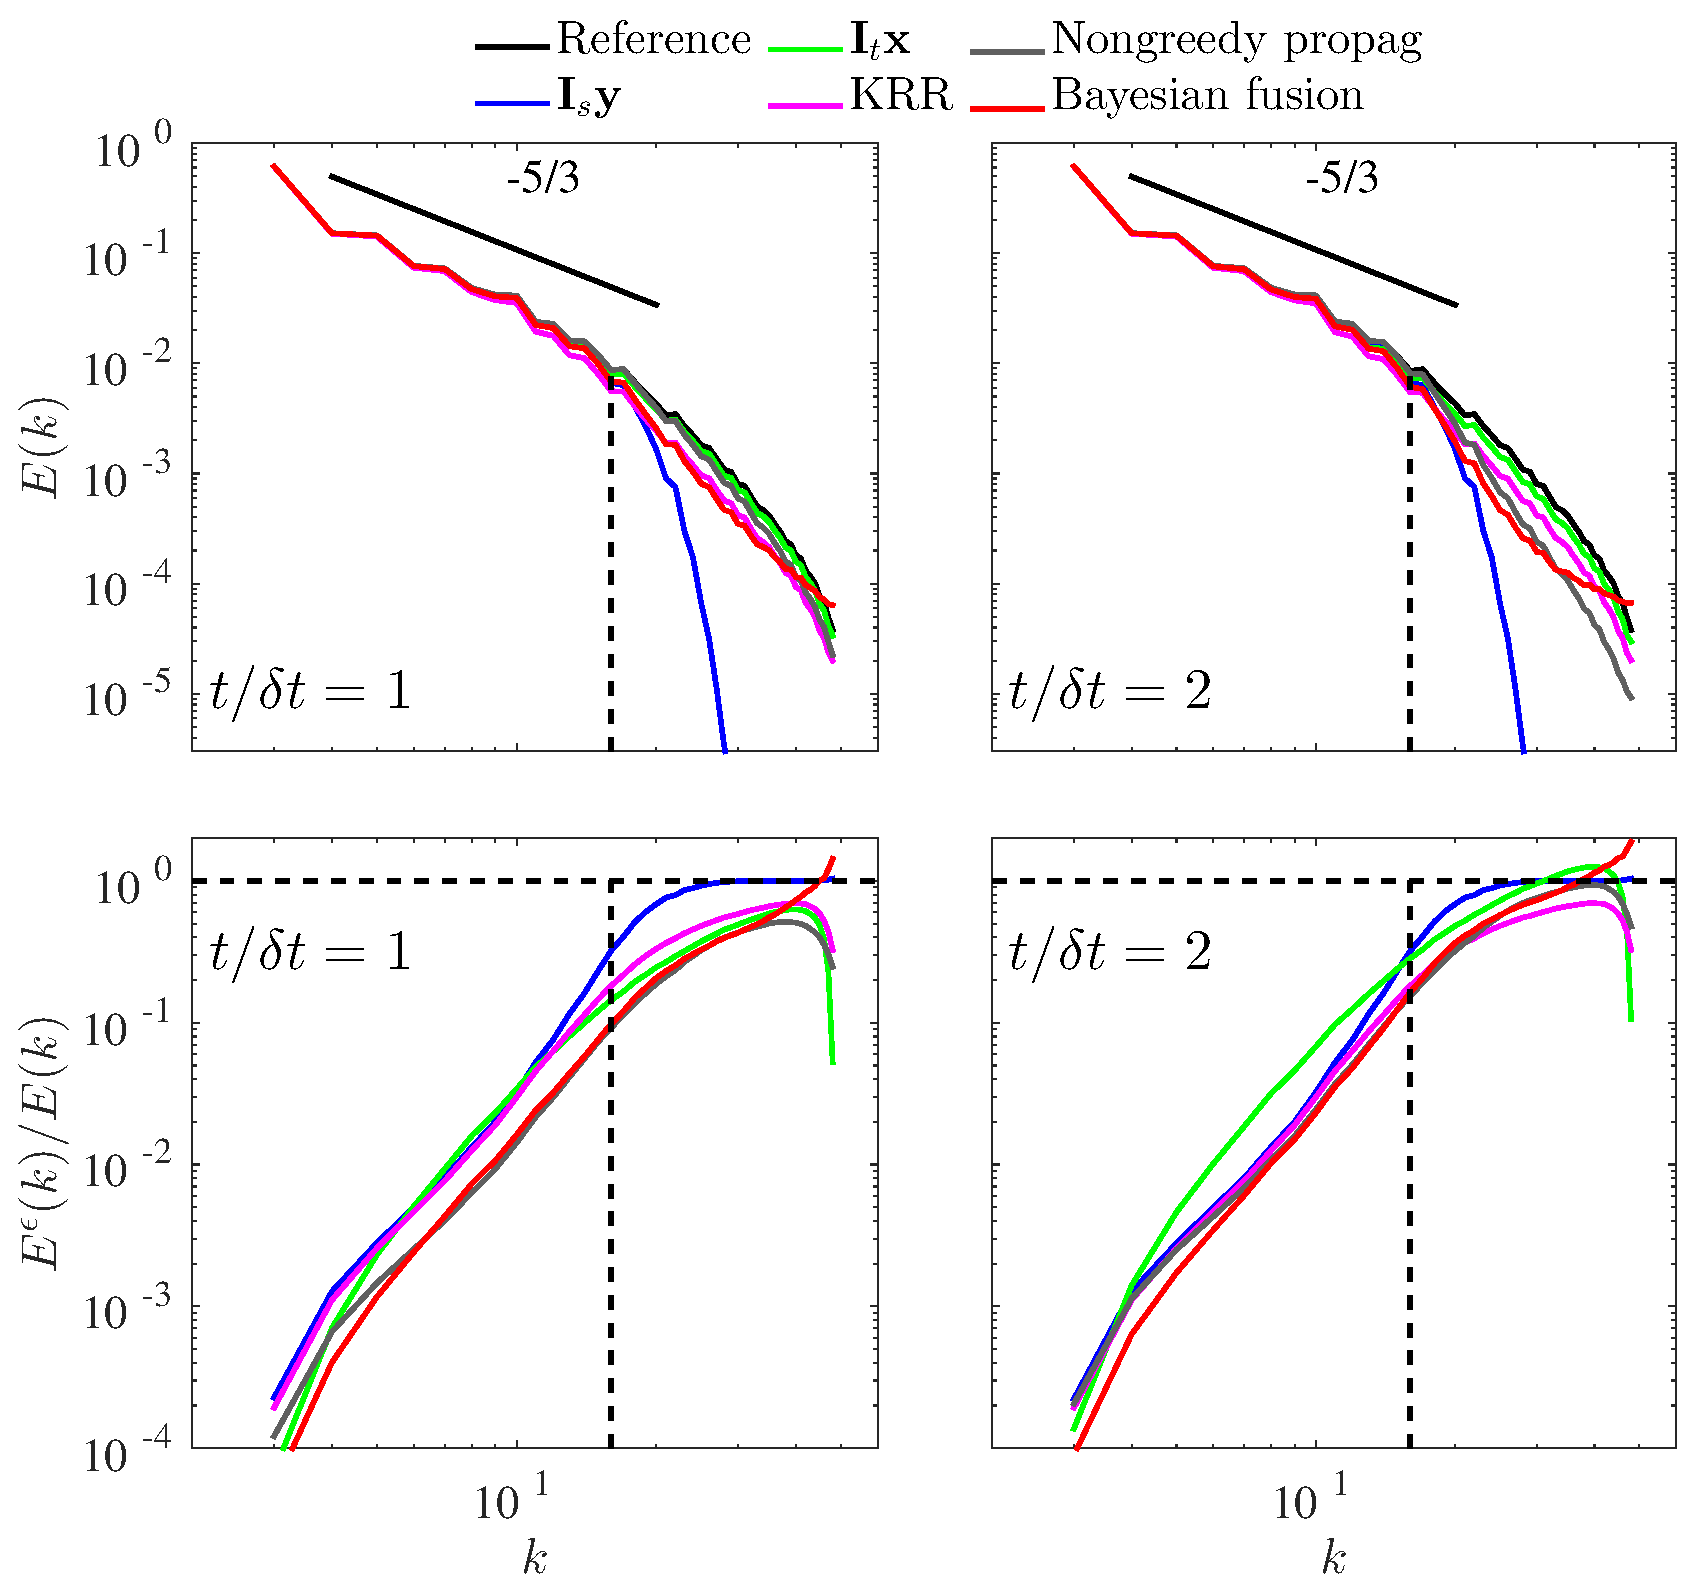
\includegraphics[width = 0.8\columnwidth]{./images/comparisons/isotropic/spectra_sspacing3_tspacing4.eps}
\caption{\label{fig:spectra_sspacing3_tspacing4} Isotropic turbulence: comparison of energy spectra and error spectra for reconstructions by interpolations (in space and time), KRR, non-greed propagation and Bayesian fusion model in case 5 of subsampling ratios $ \dimsh/\dimsl = 3 \times 3 $ in space and $ \dimth/\dimtl = 4 $ in time (see table \ref{tab:comparisons_various_cases}). The spectra are averaged over all planes of the same distance to the closest LTHS plane, i.e. $ t/\delta t = 1 $ (left) or $ t/\delta t = 2 $ (right).}
\end{center}
\end{figure}

Figure \ref{fig:spectra_sspacing3_tspacing4} shows the spectral analysis of the reconstruction by different models. To make the plot readable, RR, greedy propagation and linear Gaussian models are omitted. Energy spectra and error spectra are shown for the two positions, either close or far from LTHS planes. The first two spectra illustrate that spatial interpolation captures only large-scale information, while time interpolation gives an estimate with a good energy spectrum. All models are subject to a certain energy loss at small scales. The error spectra shows that time interpolation gives good energy spectra with poorly reconstructed small scales. KRR also shows significant improvement compared to spatial interpolation, both in energy spectra and error spectra. Compared to those that have been shown in figure \ref{fig:NLmean_interps_sspacing3_tspacing4_spectra2d}, the Bayesian fusion model Bayesian fusion model shows similar results compared to the non-greedy propagation. Both models yield compromise estimates, where certain amount of small scales are captured. Error spectra illustrate improvements at all frequencies compared to both interpolations.

\section{Reconstruction results on DNS data of channel flow}
\label{sec:comparisons_channel}
This section further analyses and compares performances of proposed methods on the DNS data of a turbulent channel flow with a moderate Reynolds number as described in section \ref{sec:data_channel}. This data mimics the experiments from WALLTURB project \citep{coudert2011double}, and simulates better practical flows compared to isotropic turbulence. Its characteristics are strongly non-homogeneous in vertical direction. The real ``time'' dimension is considered instead of a ``virtual'' one as in the previous dataset.

\begin{table}[t]
	\caption{\label{tab:final_various_cases_channel}
	Channel flow: configuration parameters of seven testing cases. The subsampling ratios of HTLS measurements are $ \sqrt{N/M} $ and equal in both spatial directions. The ratios of LTHS measurements in time are $ P/Q $. The spacing in spanwise direction is normalized by half channel height as $ \Delta z/H $ and the spacing in time is $\Delta t$, normalized by $ H/U_{max} $ ($ U_{max} $ is the central velocity of the flow). The normalized energy losses in space $\Delta\kappa_s$ and in time $\Delta\kappa_t$ are defined in Eq.~(\ref{eq:RMS_losses}).}
	\vspace{.5cm}
	\centering
	\begin{tabular}{ccS[table-format=2.0]S[table-format=2.0]cS[table-format=1.2]S[table-format=1.2]cS[table-format=1.2]S[table-format=2.2]} 
		\toprule
		\multirow{2}{*}{Case}&\multicolumn{1}{c}{}&\multicolumn{2}{c}{Subsampling ratios}&\multicolumn{1}{c}{}&\multicolumn{2}{c}{Spacings}&\multicolumn{1}{c}{}&\multicolumn{2}{c}{Energy loss}\\ 
		\cmidrule{3-4} \cmidrule{6-7} \cmidrule{9-10}
		 & & {$\sqrt{\dimsh/\dimsl}$} & $\dimth/\dimtl$ & & {$\Delta z/H$} & {$\Delta t$} & & {$\Delta\kappa_s(\%)$} & {$\Delta\kappa_t (\%)$}\\ 
		\midrule 
		5 &  & 05  & 04 & & 0.05  & 0.10 & & 1.23 & 1.88 \\ %\addlinespace	 
		6 &  & 10  & 10 & & 0.11  & 0.25 & & 7.08 & 9.02 \\ %\addlinespace
		7 &  & 20  & 20 & & 0.22  & 0.50 & & 20.83 & 24.31\\ %\addlinespace
		\bottomrule
	\end{tabular}
\end{table}


\begin{table}
\caption{\label{tab:final_results_channel}
Channel flow: NRMSEs of all scales reconstruction errors for three cases in Table.~\ref{tab:final_various_cases_channel}. $\overline{\epsilon}$ and $\epsilon_{max}$ are the mean and max NRMSE defined in Eq.~(\ref{eq:NRMSE}). $\overline{\epsilon}$ is averaged over all space-time positions in the outer region $ y/H \in [0.25,1.75] $, while $\epsilon_{max}$ is computed for one of the most difficult position in space and time (the most remote from all nearby measurements). The smallest errors in each cases are boldfaced.}
\vspace{.5cm}
\centering
	\begin{tabular}{lcccccccc} 
		\toprule \multirow{2}{*}{Method}&\multicolumn{1}{c}{}&\multicolumn{3}{c}{$\overline{\epsilon}$}&\multicolumn{1}{c}{}&\multicolumn{3}{c}{$\epsilon_{max}$}\\
		\cmidrule{3-5} \cmidrule{7-9}
		 & & {Case 5} & {Case 6} & {Case 7} & & {Case 5} & {Case 6} & {Case 7}\\
		\midrule 
		$ \Interp_s \y $ & & 0.14 & 0.36 & 0.68 & & 0.16 & 0.47 &  0.85 \\ 
		$ \Interp_t \x $ & & 0.11 & 0.32 & 0.54 & & 0.18 & 0.55 &  0.85 \\
		RR & & 0.12 & 0.34 & 0.64 & & 0.15 & 0.49 &  0.78 \\
    	Fusion (BF)  & & 0.08 & 0.25 & 0.46 & & 0.13 &  0.43 &  0.73 \\ 
    	\midrule
    	\myrowcolour
    	Best scores  & & \textbf{0.08} & \textbf{0.25} & \textbf{0.46} & & \textbf{0.13} &  \textbf{0.43} &  \textbf{0.73} \\ \bottomrule
	\end{tabular}
\end{table}

Based on the analyses on isotropic turbulence, and for simplicity, only RR and Bayesian fusion model are selected to represent the two families of approaches. Three cases of balanced subsamplings in space and time are considered. The configurations with subsampling ratios, spacings and amounts of energy loss are presented in table \ref{tab:final_various_cases_channel}. The losses in space (2D) and time are similar in each case, from very small energy losses (less than $ 1 \sim 2 \% $ in case 5) to very severe ones (more than $ 20 \% $ in case 7). The average and maximum NRMSEs of reconstructions by all methods for the three cases are shown in table \ref{tab:final_results_channel}. The best errors obtained by the fusion model are boldfaced and shown in the last row. 


\begin{figure}
\begin{center}
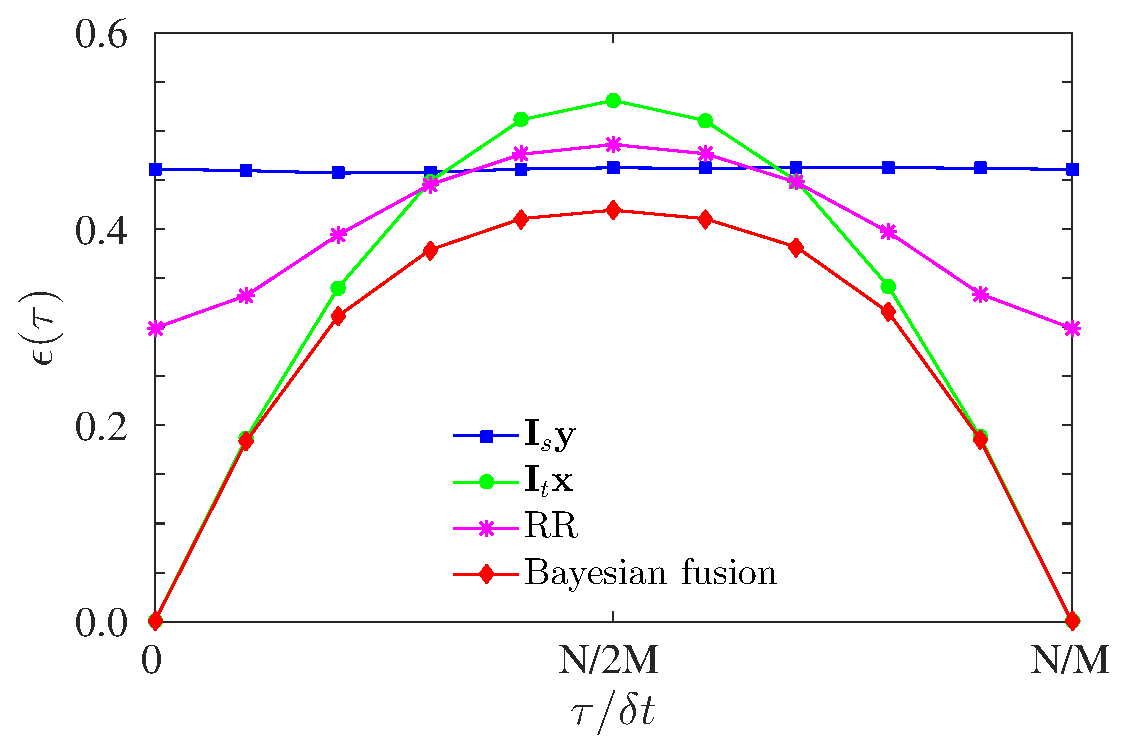
\includegraphics[width = 0.8\columnwidth]{./images/comparisons/channel/error_MAP_newOM1_middlepoint_outer.eps}
\caption{\label{fig:final_channel_error_time} Channel flow: NRMSEs between reference and reconstructed streamwise velocities by all methods as: functions of time distances from the previous LTHS instant at the most difficult spatial location, i.e. at $ (\Delta y/2,\Delta z/2,\tau) $. Results are shown for case 5 in table \ref{tab:final_various_cases_channel}, with the subsampling ratios $ \dimth/\dimtl = 10 $ in time and $ \dimsh/\dimsl = 10 \times 10 $ in space.}
\end{center}
\end{figure}

\begin{figure}
\begin{center}
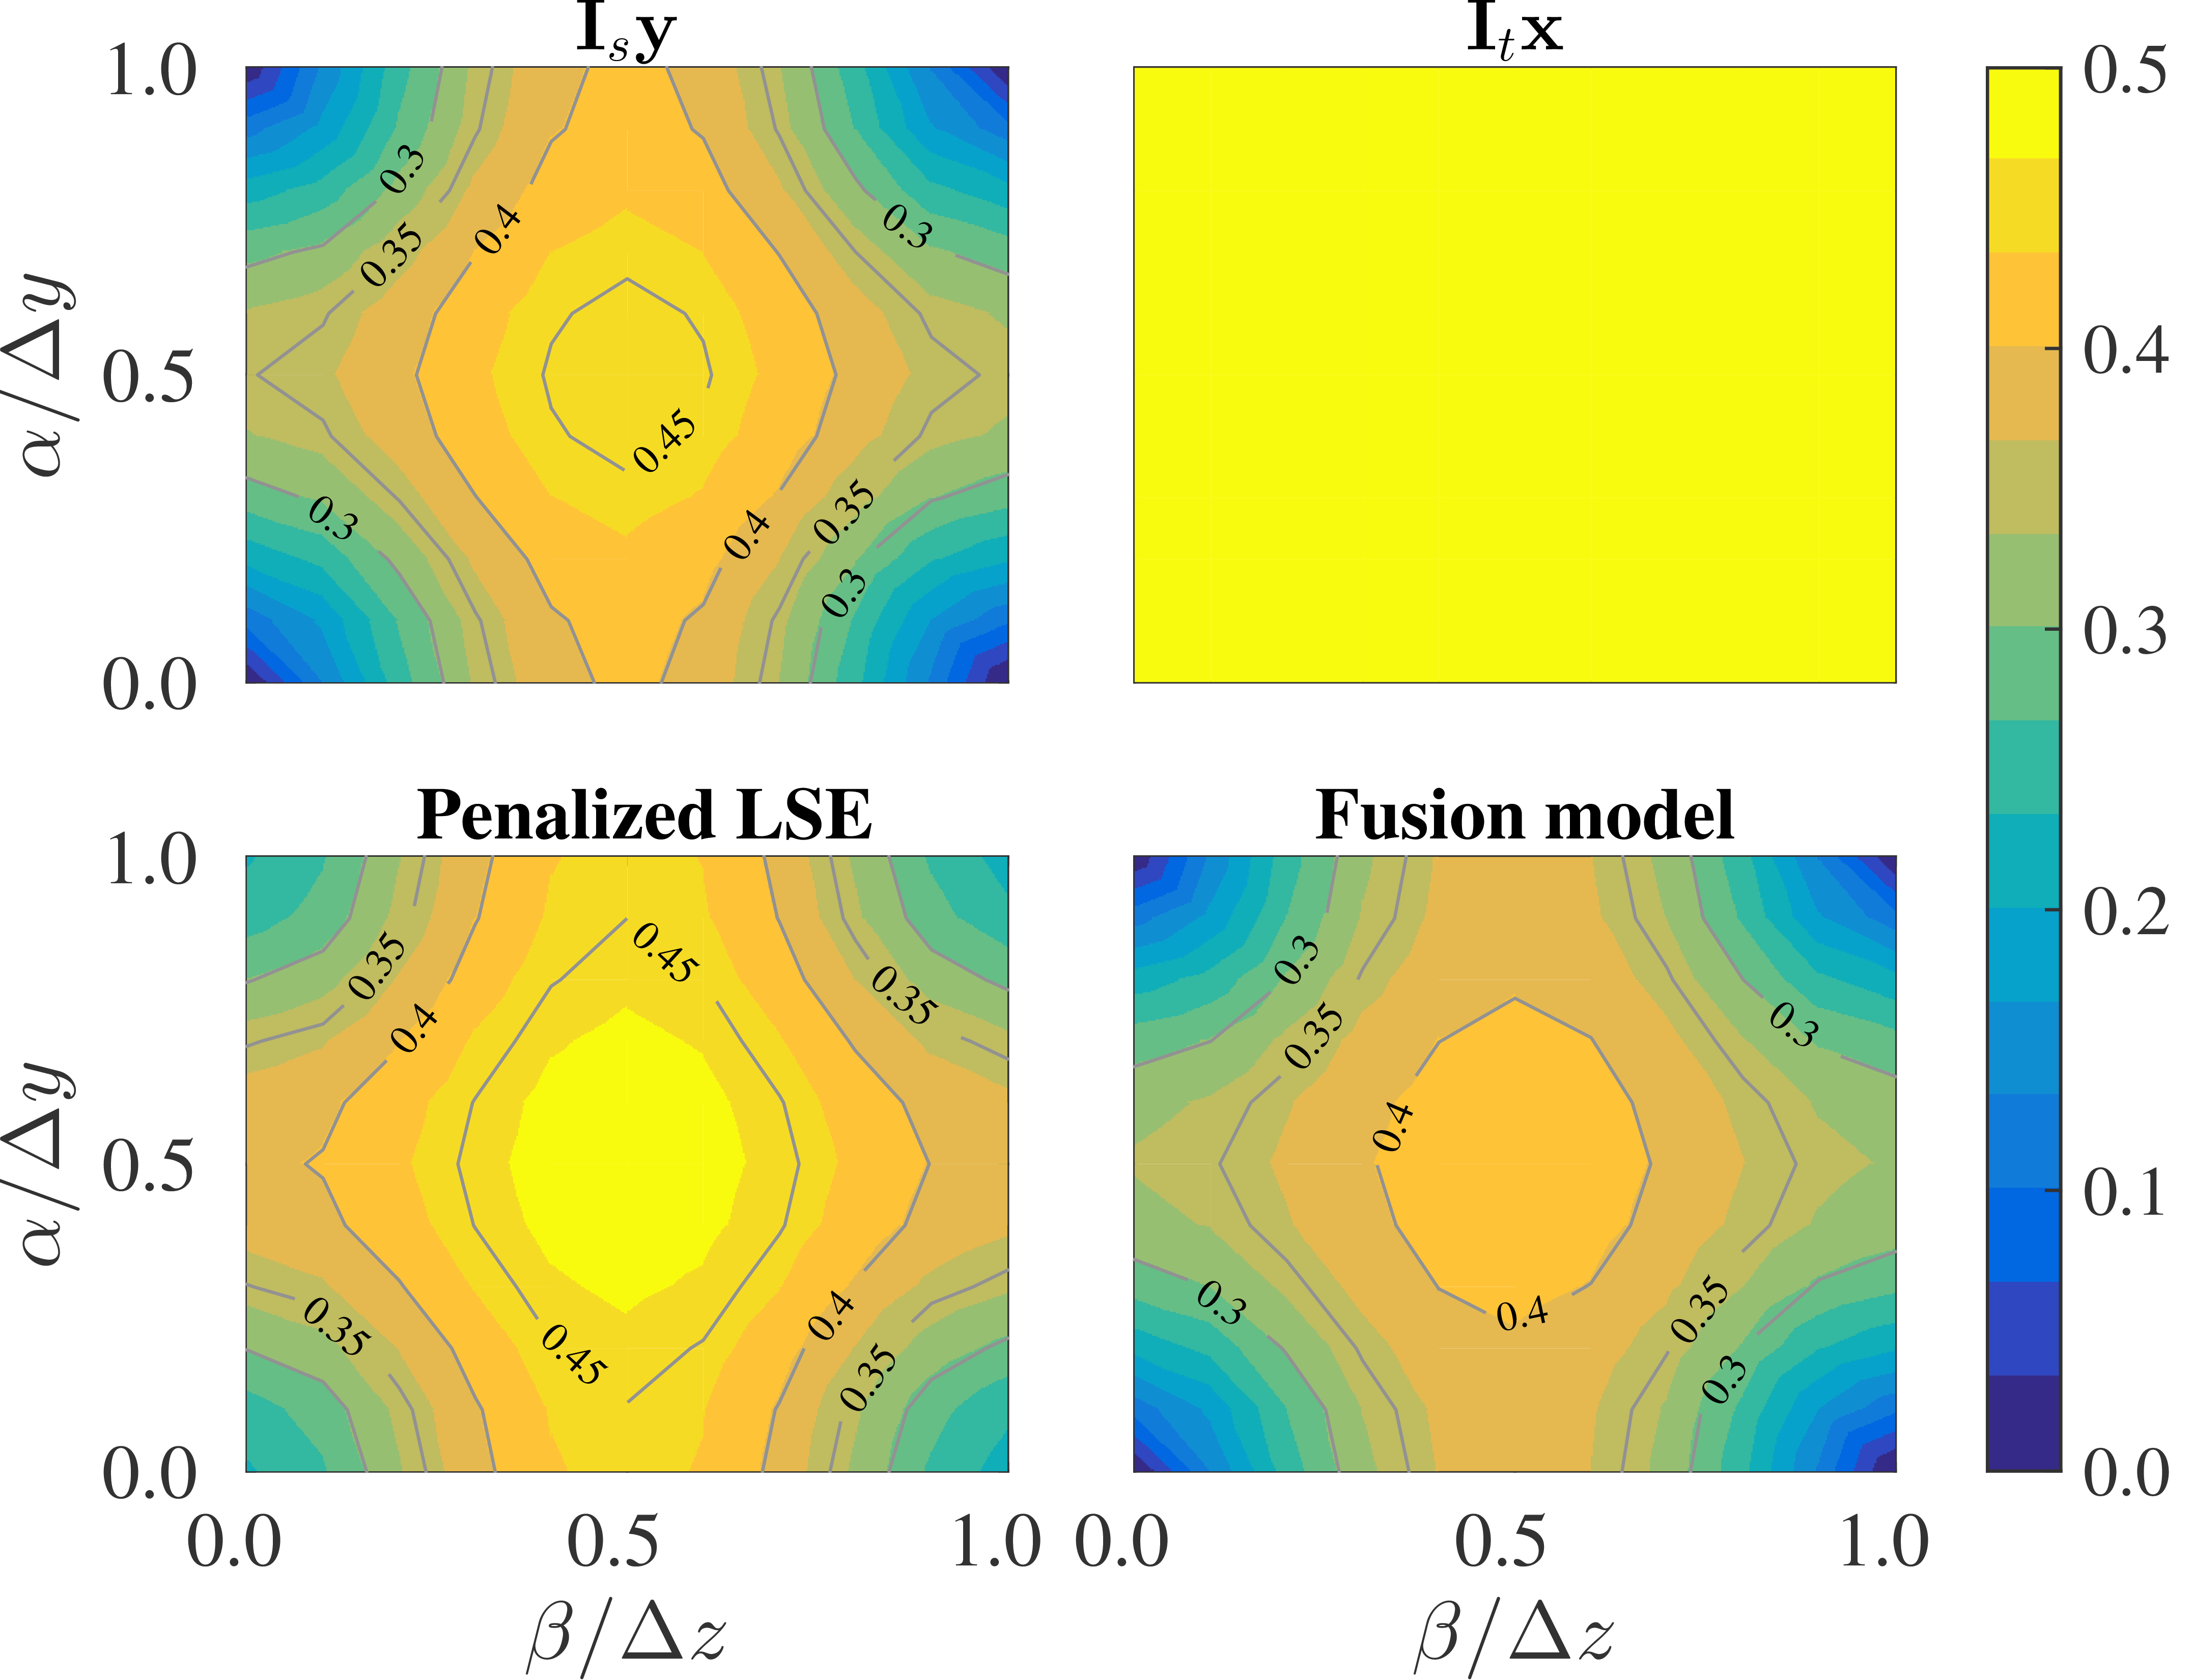
\includegraphics[width = 0.8\columnwidth]{./images/comparisons/channel/error_MAP_newOM1_boxin4HWs_outer.png}
\caption{\label{fig:final_channel_error_boxes} Channel flow: NRMSEs between reference and reconstructed streamwise velocities by all methods as: functions of spatial coordinates in an element block at the most difficult instant, i.e. at $ (\alpha,\beta,\dimth \delta t/2\dimtl) $. Results are shown for case 5 in table \ref{tab:final_various_cases_channel}, with the subsampling ratios $ \dimth/\dimtl = 10 $ in time and $ \dimsh/\dimsl = 10 \times 10 $ in space.}
\end{center}
\end{figure}



Case 6 of moderate energy loss (about $ 8 \% $) is used for further visualization of the analysis. The energy losses are not too severe but are critical to highlight interests of the present approach. $ \overline{\epsilon} $  and $ \epsilon_{max} $ are reduced by 25 $ \% $ and 35 $ \% $ respectively for all scales reconstruction. Model performances in time and in space are shown in figures \ref{fig:final_channel_error_time} and  \ref{fig:final_channel_error_boxes}respectively. They are estimated and plotted similarly as in figures \ref{fig:final_isotropic_error_boxes_case7} and \ref{fig:final_isotropic_error_time_case5}. The fusion model clearly demonstrates the benefits of combining information in space and time by proposing a compromise estimate from the two single interpolations. 


\begin{figure}
\begin{center}
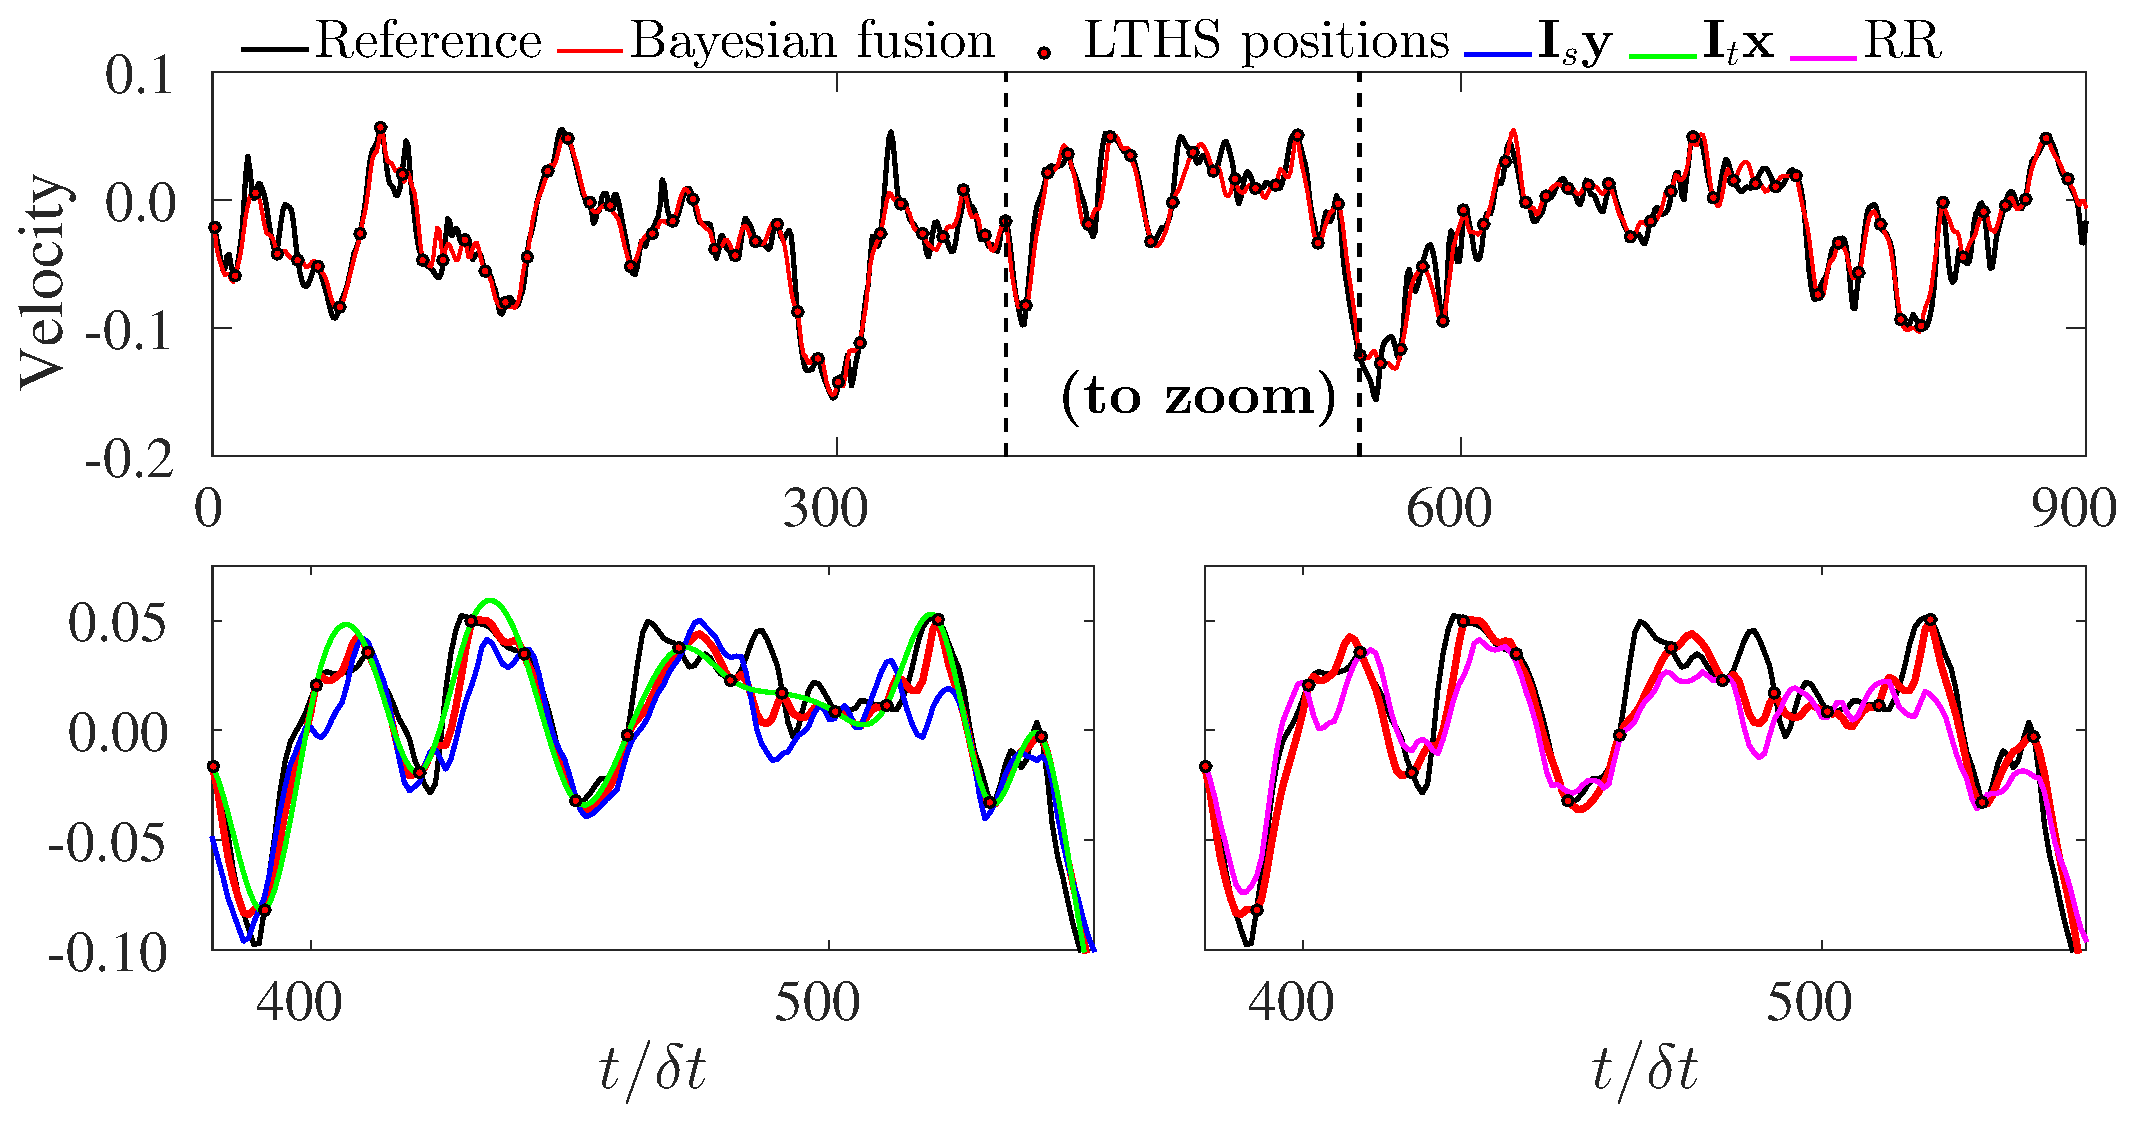
\includegraphics[width=\columnwidth]{./images/comparisons/channel/improper_point_spacespacing_10_timespacing_10_yid129_zid149.eps}
\caption{\label{fig:final_channel_timeseries} Channel flow: a time evolution of fluctuating streamwise velocity at $ y/H=1 $ and $ z/H=0 $ of a point with the local coordinate $ (\Delta y,\Delta z, \tau) $  (see figure (\ref{fig:element_block}) ). The whole evolutions of reference and fused velocity contain $ 900 $ samples. A region is zoomed in and compared with results from interpolations and RR.}
\end{center}
\end{figure}

Figure \ref{fig:final_channel_timeseries} shows a time evolution of the point at $ y/H=1 $ and $ z/H=0 $ ($ \alpha=\Delta y /2 $ and $ \beta = \Delta z/2 $ in local coordinates, see figure \ref{fig:element_block}), the most remote from neighboring HTLS sensors. A good agreement between fused and reference velocity is still obtained. A zoom-in period is shown for detailed comparisons with other methods. While time interpolation captures only low frequencies, spatial interpolation generates high frequencies but weakly correlated with the truth. The fusion model proposes a good compromise to improve both large and small scales reconstruction. It also captures detailed peaks much better than RR, since RR smooths these small scales out by minimizing the mean square errors. 

\begin{figure}
\begin{center}
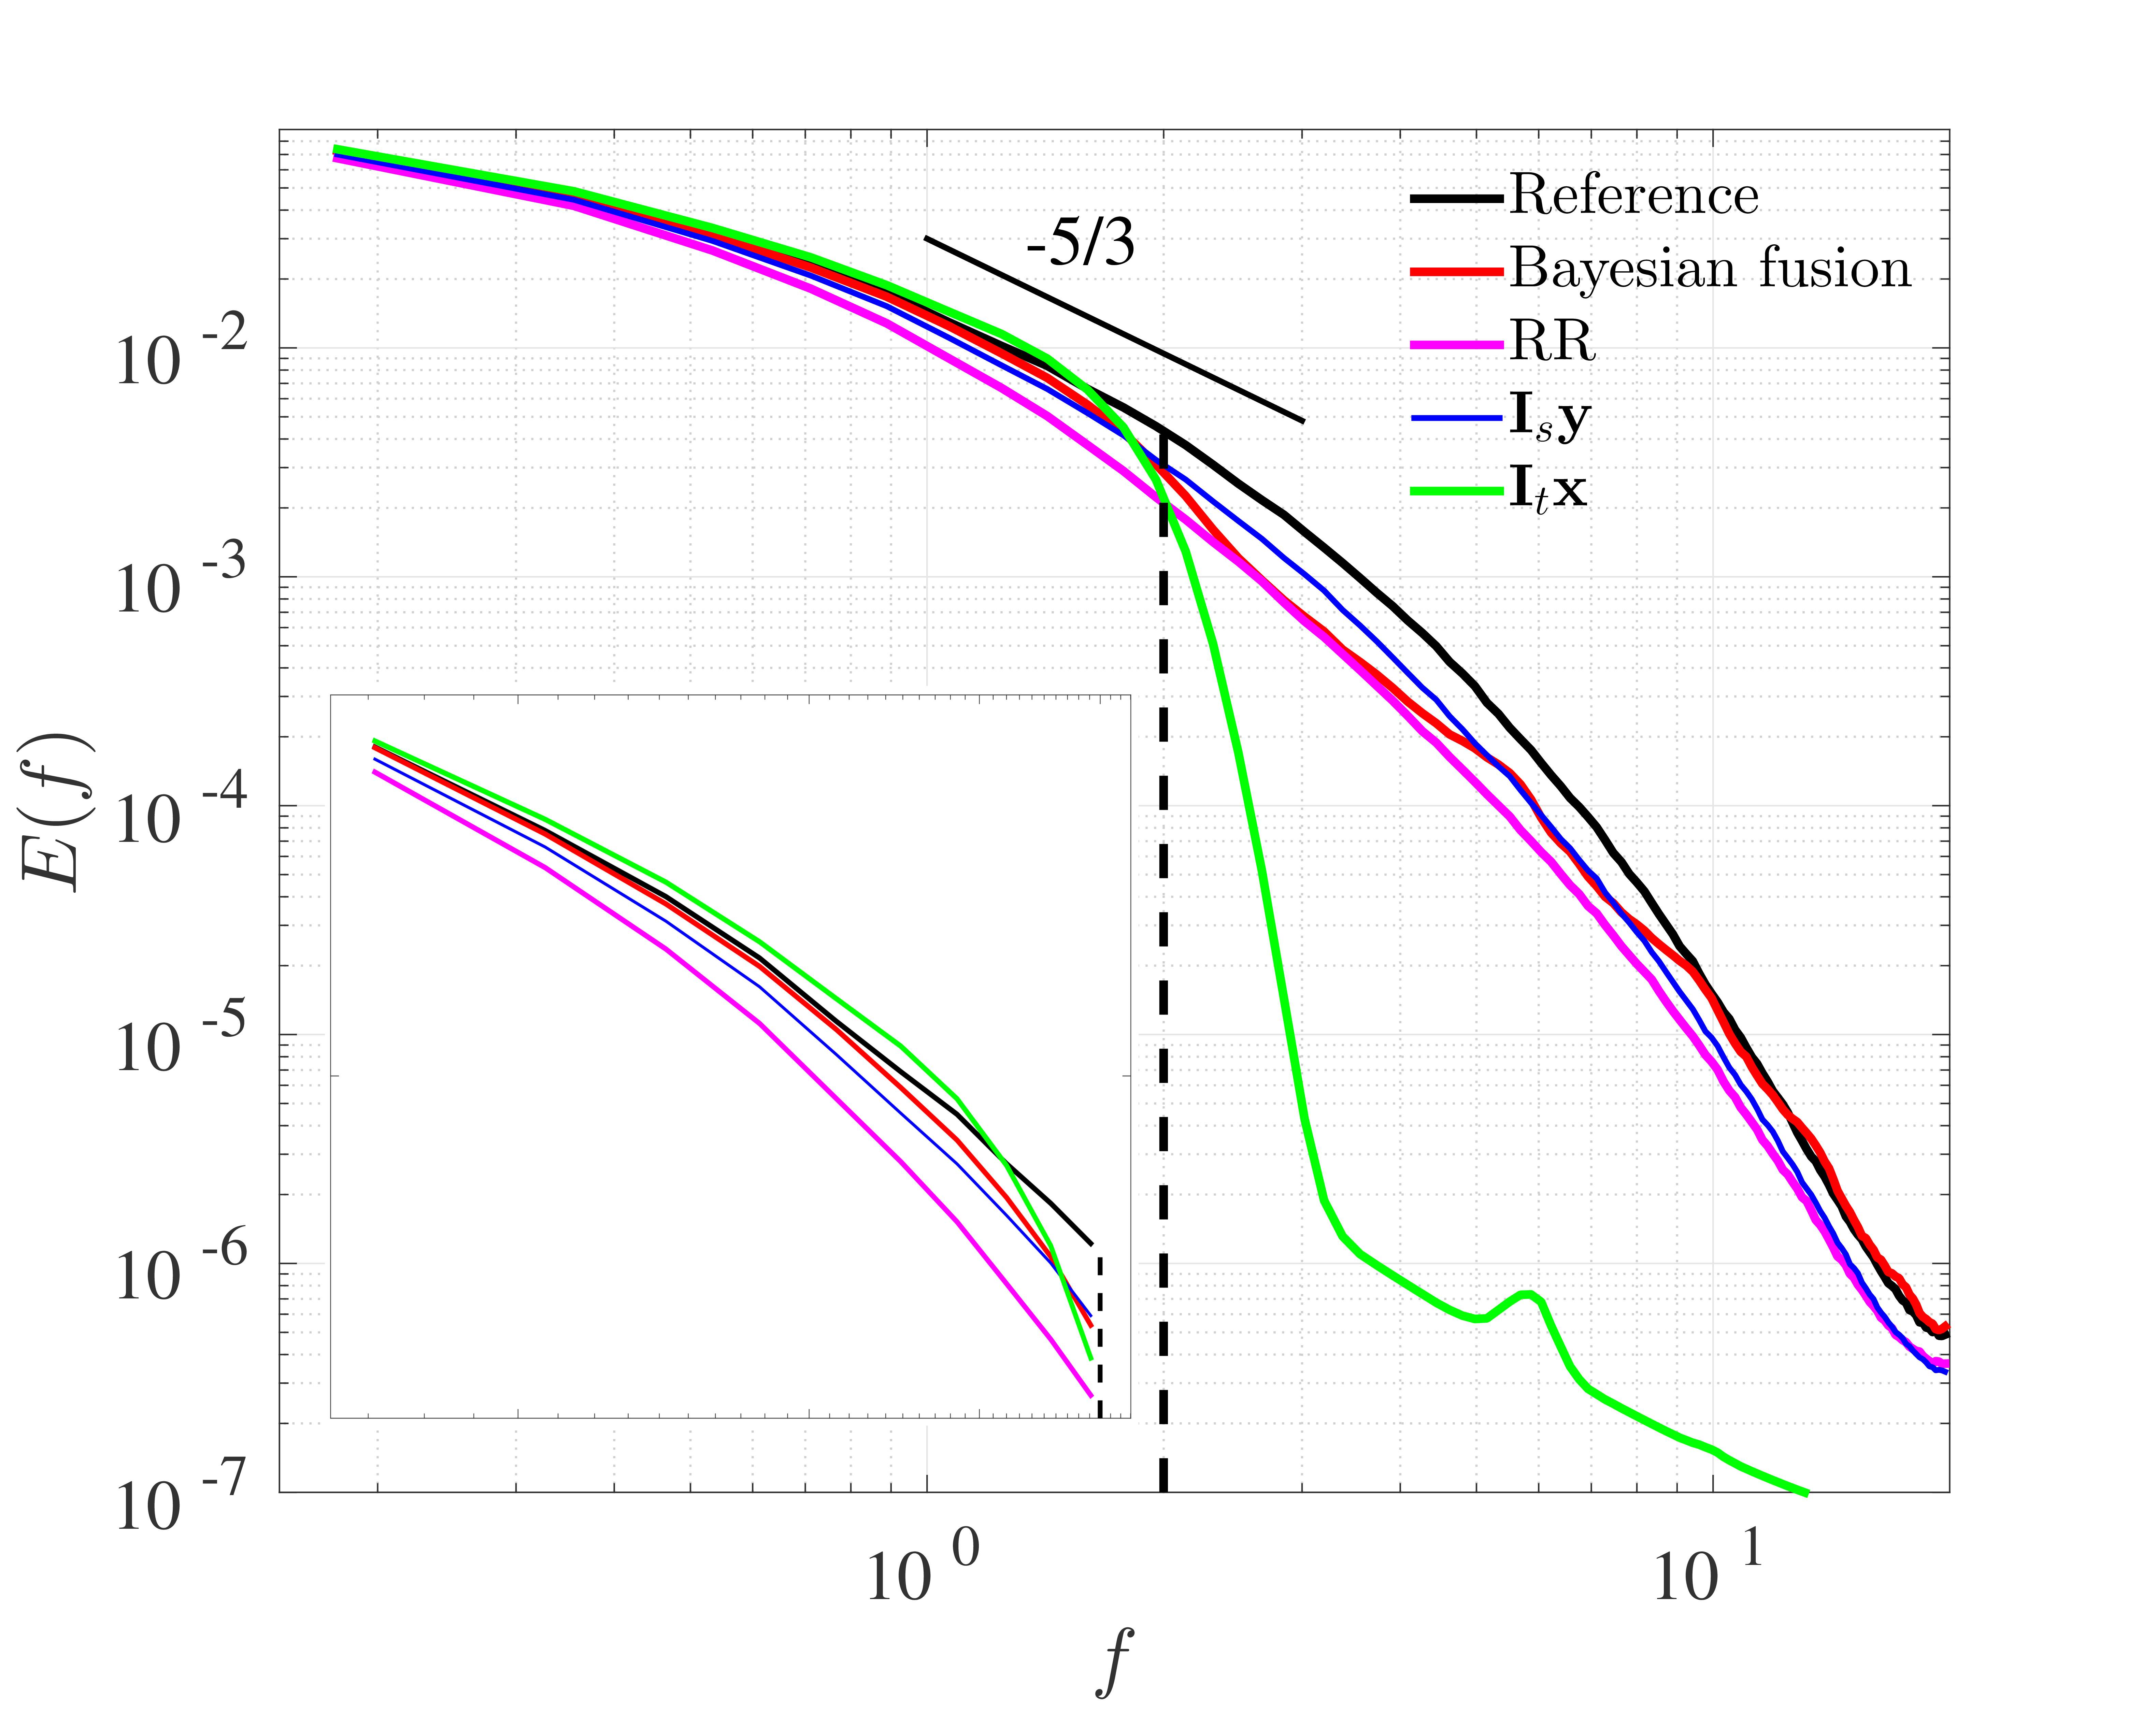
\includegraphics[width=0.8\columnwidth]{./images/comparisons/channel/improper_sspacing_10_tspacing_10_spectrum_time_joint.png}
\caption{\label{fig:final_channel_spectra} Channel flow: spectra of the fluctuating velocity in figure \ref{fig:final_channel_timeseries}.}
\end{center}
\end{figure}

Temporal spectra, estimated from the same points as those shown in figure \ref{fig:final_channel_timeseries}, are compared in figure \ref{fig:final_channel_spectra}. Time interpolation fails to estimate the signal at higher frequencies than a certain cutoff. RR reconstructs both large and small scales, but the loss of large scale energy is critical. This loss is highlighted in the zoom-in picture of low frequencies. The present model improves the estimation at both low and high frequencies.

\begin{figure}
\begin{center}
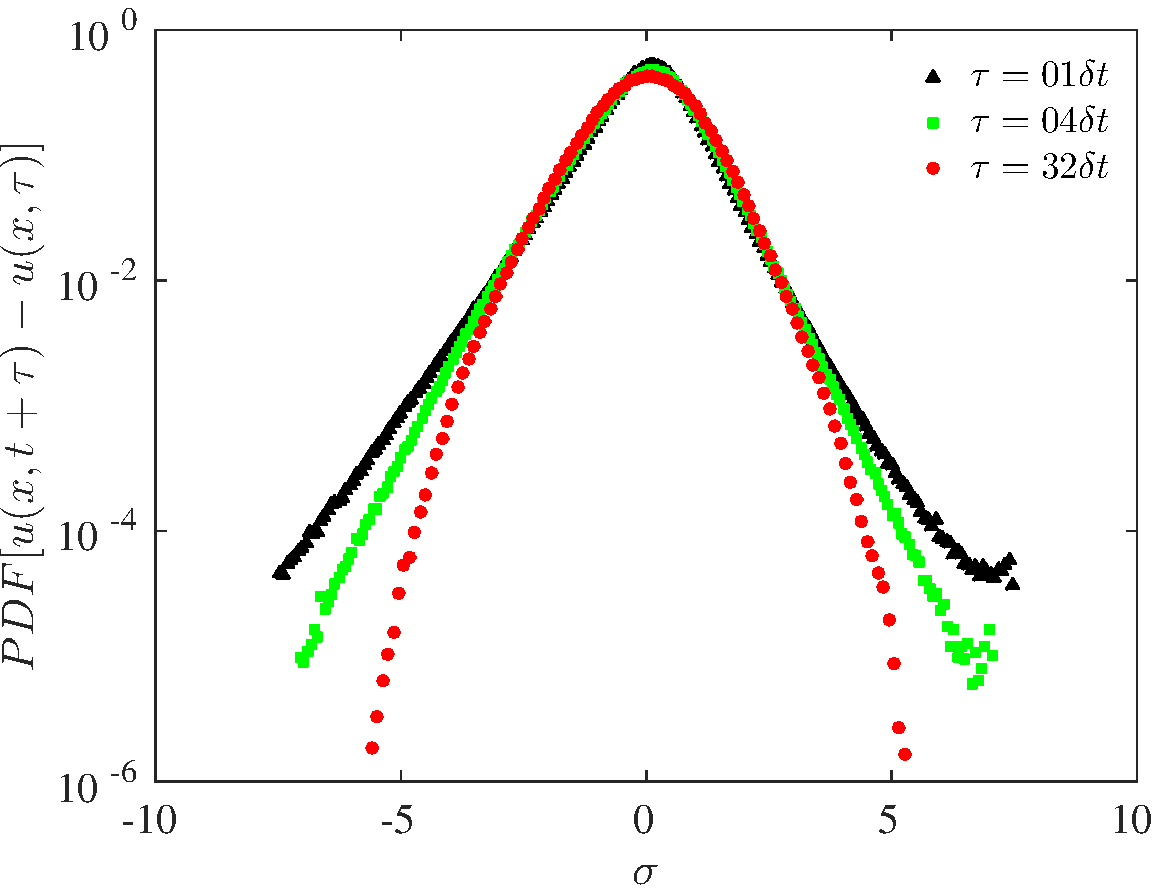
\includegraphics[width=0.49\columnwidth]{./images/comparisons/channel/pdf_org}
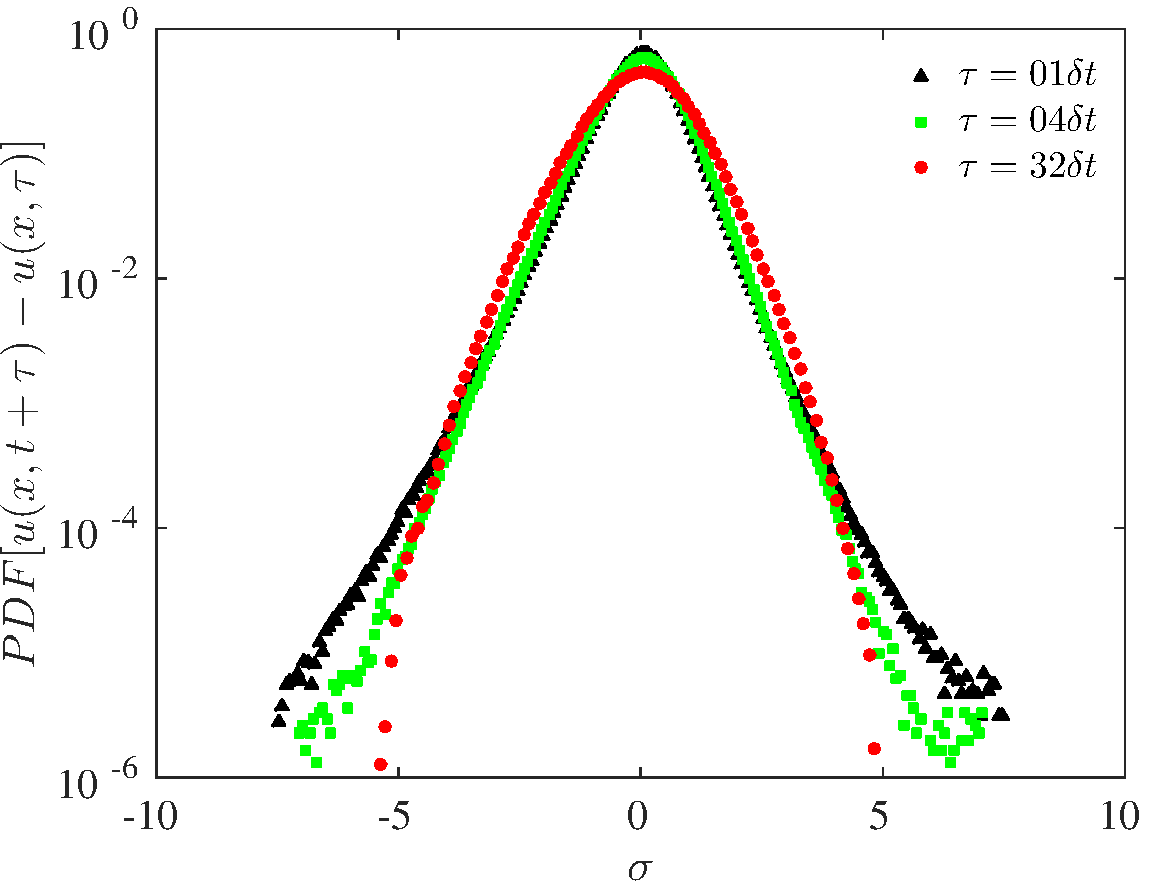
\includegraphics[width=0.49\columnwidth]{./images/comparisons/channel/pdf_fusion}
\caption{\label{fig:final_channel_pdf} Channel flow: probability distribution functions of velocity increments in (left) the original DNS and (right) the reconstructed field.}
\end{center}
\end{figure}

Figure \ref{fig:final_channel_pdf} shows estimates of the probability density functions of time increments $u(x,t+\tau)-u(x,t)$ for the original DNS field as well as for the reconstructed field. As expected, the original field displays intermittent non Gaussian distributions. More importantly, the reconstructed field, while less intermittent, still clearly exhibits non Gaussian increments at small scales. Note that the reconstruction error is essentially due to the difficulty to accurately reconstruct these small scales. It is expected that any reconstruction method will lead to fields that are less intermittent than the original one.

\begin{figure}
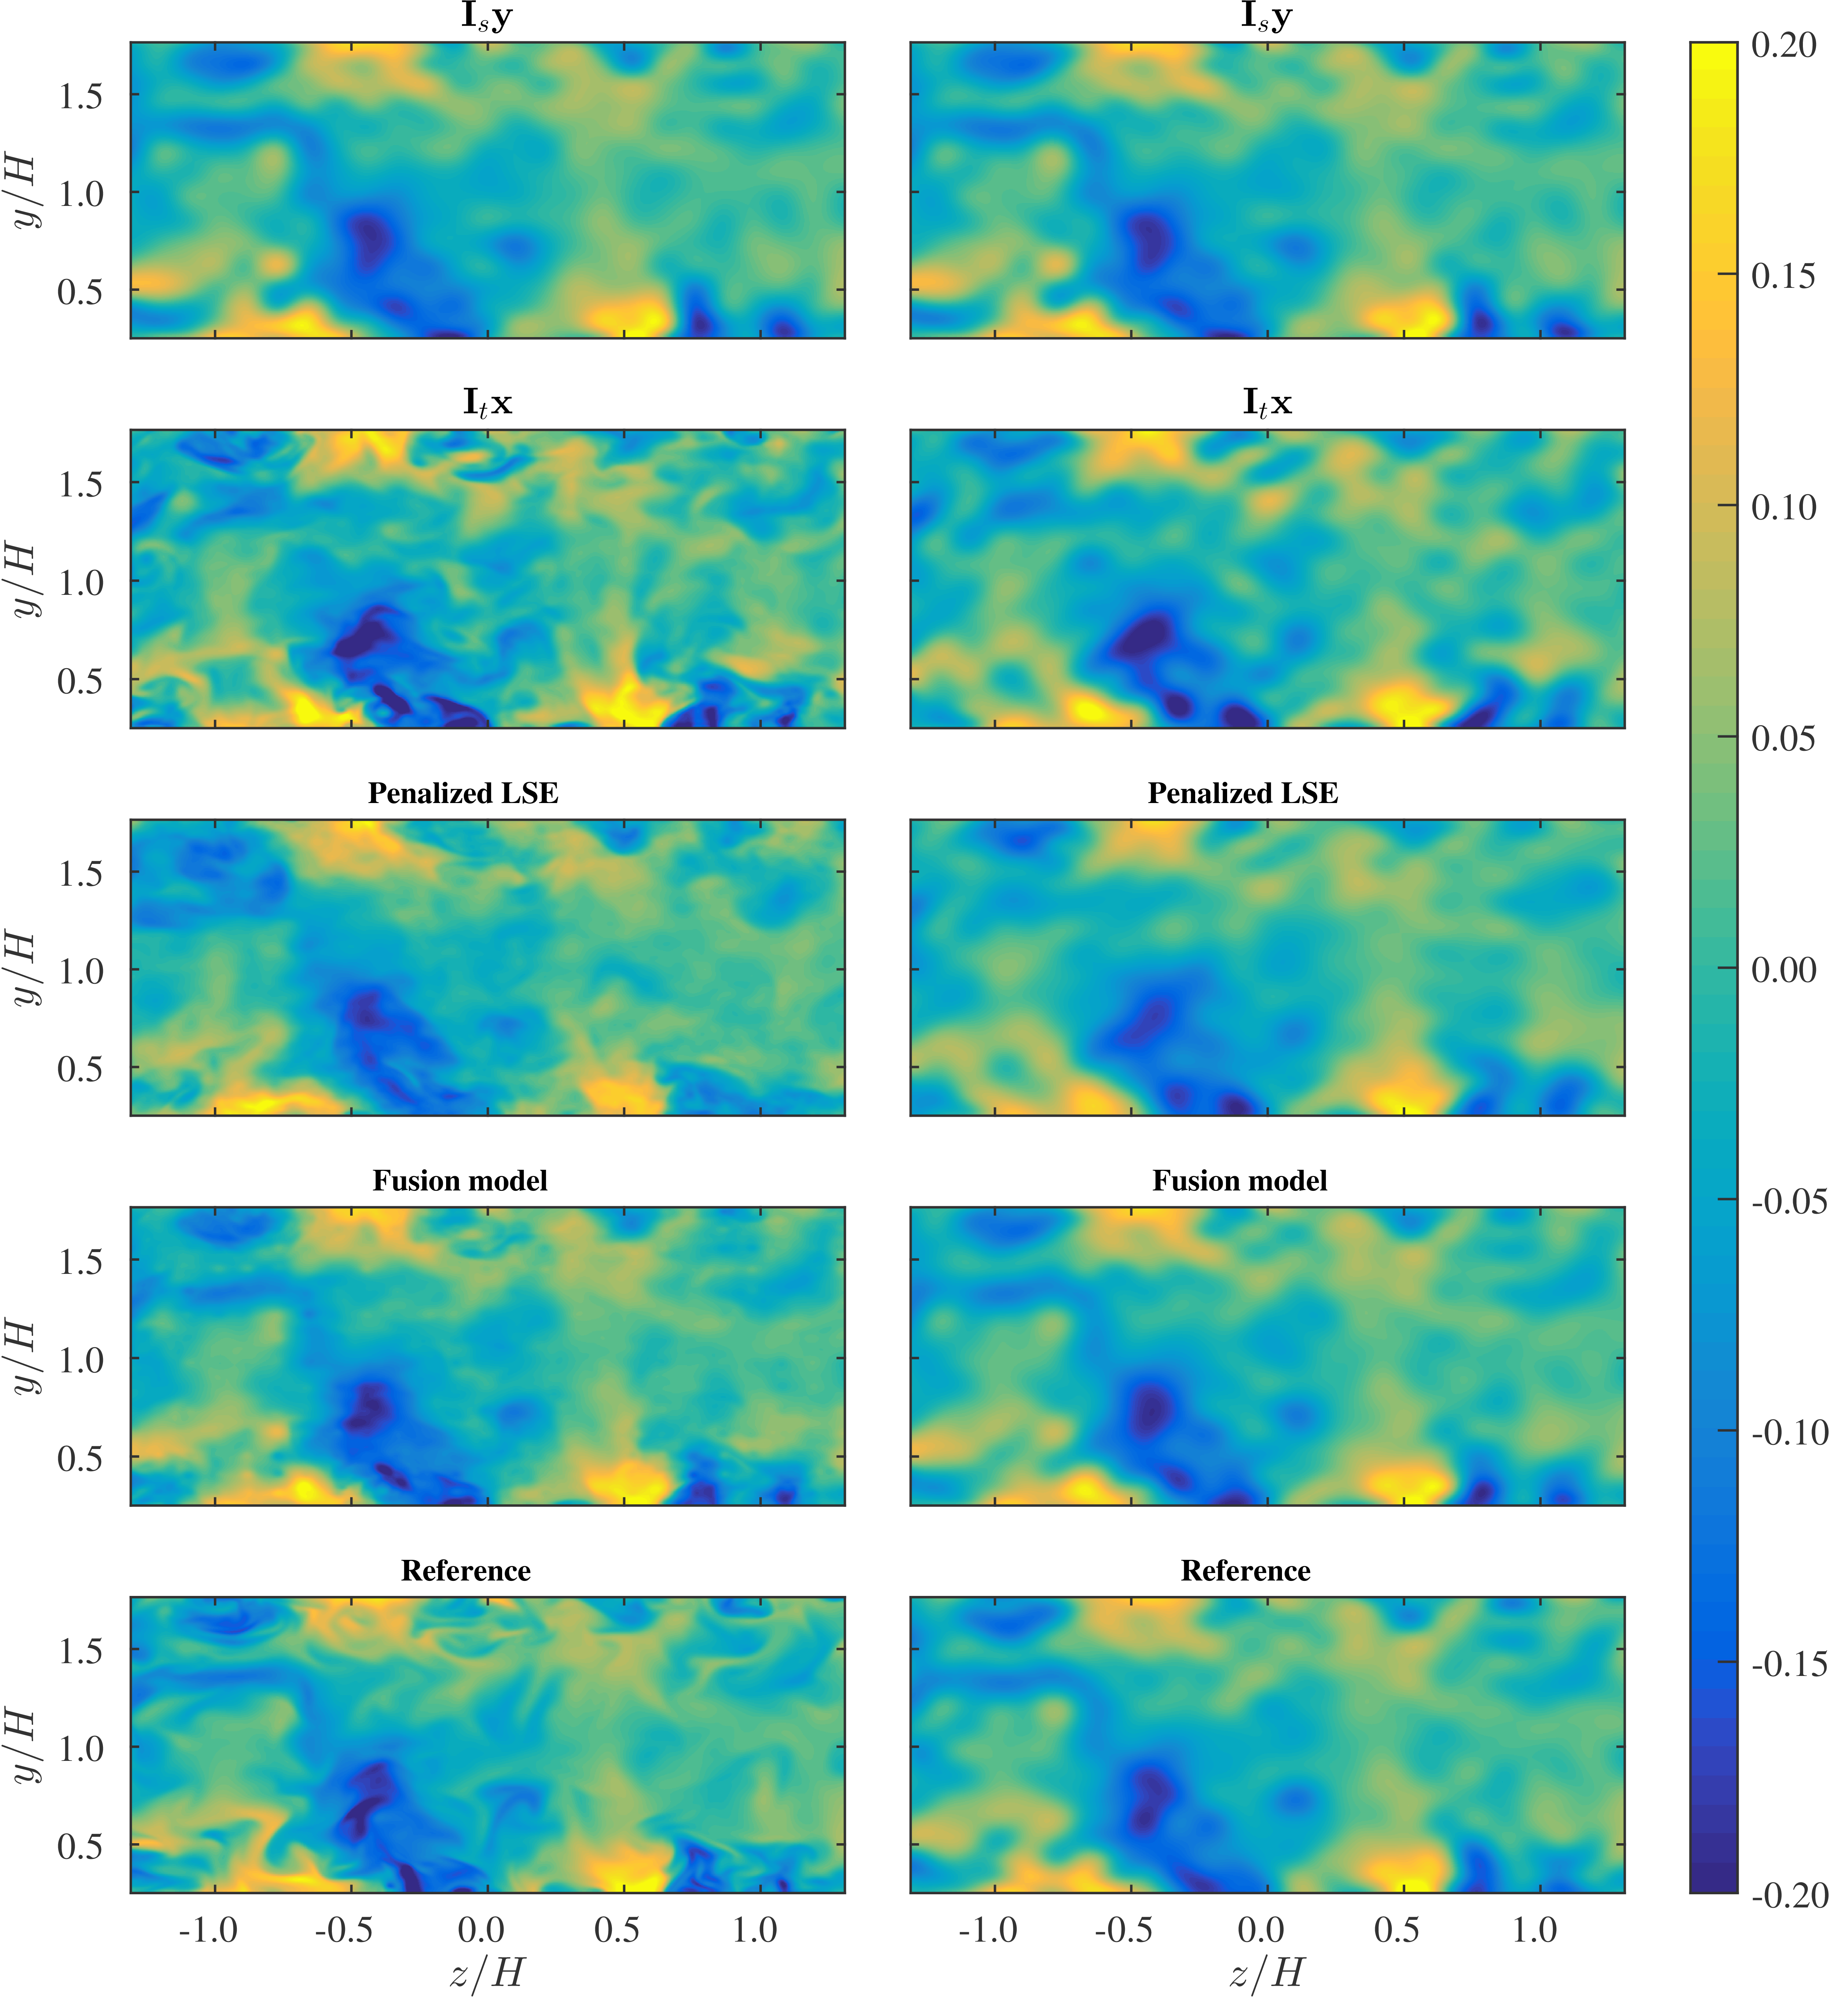
\includegraphics[width=\textwidth]{./images/comparisons/channel/improper_outer_spacespacing_10_timespacing_10_subplots_all_t006.png}
\caption{\label{fig:final_channel_fields} Channel flow: a sample snapshot of fluctuating streamwise velocity at one of the most difficult instant to estimate (in the middle of two LTHS time steps): Reconstruction of all scales (left) and large scales only (right). The figure is better viewed on screen.}
\end{figure}

Figure \ref{fig:final_channel_fields} compares reconstructed snapshots by different methods. This snapshot is at the most remote instant from its two neighboring LTHS time steps. The model reconstructs correctly the velocity field with more flow details than spatial interpolation. It also recovers better large scales than RR and time interpolation methods.

\section{Concluding remarks}
This section analyzes performances of all the models discussed in this thesis. All reconstructions are gathered and compared to highlight the behaviors of different models. These comparisons also suggest further ideas to improve the models by combining several of them to take advantage of different sources of information. 

Two datasets have been used, the DNS data of an isotropic turbulence and a turbulent channel flow at a moderate Reynolds number. Only the streamwise velocity component is studied, but all results can be reproduced for other components. In all configurations, HTLS and LTHS measurements are used as complementary information in space and time. Empirical models find the relation between large and small scales, while fusion models combine two sources of measurements. Only the cases of balanced energy losses are investigated, since otherwise fusion models give results similar to single interpolation of the measurements with the lower energy loss.

Performances of regression models depend only on the subsampling ratio in space. This was expected since these models are not designed to take advantage of information in time. The benefits of such models are highlighted only in comparison to spatial interpolation. The improvements are significant. Kernel regression models also show their superiority compared to linear ones. This is certainly due to the non-linear relation between large and small scales in turbulence.

NLM-based propagation models reconstruct the small scales using a different prior. Small scales are assumed to be advected by larger ones. These small-scale information are then propagated along the time direction based on the similarity levels of corresponding large scales in space. Results show some advantages especially when the subsampling ratios are small in both space and time. A ratio of $ 3 \times 3 $ in space, corresponding to about $ 1\% $ of energy loss, ensures that the model does not start from a too severe loss of information. In time, a ratio of $ 4 $, also about $ 1\% $ of energy loss, ensures that the similarity level between large scales remains significant. Significant benefits are observed compared to spatial interpolation, even in rather crude subsampling ratios in space and time. A non-greedy scheme, by gradually propagating small scales from LTHS planes, gives slightly better reconstructions compared to the greedy one. 

The analyses show advantages of further exploiting information in time. The Bayesian fusion model, despite its simplicity, demonstrates clear benefits compared to other methods. By simply proposing compromise estimates between the two interpolations in space and time, it leads to more accurate reconstruction at all positions in space and time. The compromise is achieved in the form of a weighted average, where weights are learned from measurements. These weights encode some information about the physics of the flow. Benefits are significant in cases of balanced energy losses. The 2D fields or 1D signal comparisons also demonstrate that the fusion model seeks a trade-off between retaining good large-scale information from a single interpolation and proposes more details from the other interpolation.

All models reconstruct the fields using different priors, i.e. exploiting information differently. Comparisons show clear advantages of combining different measurements. Further exploitations and combinations of such models can improve the reconstruction results. For instance, NLM-based propagation could start from initial large scales obtained from regression, which are more accurate than spatial interpolation. This propagated information, which exploits the local similarity of the flows, could combine with the time interpolation to further improve results of Bayesian fusion models. 

